%What
%Why
%How...
%diagram (?)
% overview
% road map
% how the ideas in the chapter fit together
% it should be balanced...
\label{Chapter10}
\chapter{Gas phase xenon detector for wire testing}



\subsection{Test Mass}
There are  photomultiplier tubes(PMT)

\bigskip

\noindent




\subsection{Gas circulation system}
 

\section{Sparking in the system}


\subsection{The sparking on the high voltage feed through connectors}

\subsection{The sparking on the cable grounding terminations}

\subsection{The sparking between the grids}


\section{Light propagation Simulations}
\subsection{Light creation}
(original text) There are three kind of light creation resources in the detector that is able to be collected by the PMT readout system: 1) dark current from PMT photo cathode and diodes, 2) background light from the material of the detector and outside detector region, 3) scintillation xenon light coming from an event happened in the detector region. Among these, the third one includes the electron emission events that we want to study. The first light resource is mostly thermionic emission from the PMT photo cathode material, which normally has low work function to achieve high photo electron conversion efficiency for the PMT tube. Because of each thermionic emission is independent event, dark current normally comes in forms of single electrons. So even though these type of light is dominant. However, a series of dark current event may look like a real event and contribute to false classifying event rate(false coincidence event). The second light resource has varies origins. During the sparking test, we observe visible light along with discharge coming from the high voltage feed through connectors, high voltage cable termination connectors, and high voltage cables, etc. These discharge current originated from the imperfect points on the metal surface generate xenon scintillation light outside the detector region. This current grows exponentially(following Fowler Nordheim field emission equation) with the electric field on the metal surface. However, the light collection efficiency on the outside detector region is low. Thus, an event with several photons from outside detector region also looks like a electron emission event. But, the event of electron emission from the grids have a more specified time span from the drift time of the electron between the two grid planes. We can distinguish these two type of events from these features. This feature can be use for distinguishing this background. Fluorescence light from the PTFE surface were also observed. Fig: \ref{fig: PTFE fluorescence ignition}, shows the decaying of PTFE fluorescence. To reduce this background, sparking is avoiding for emission studying. Three-day waiting time for quieting the detector was taken before each measurement. 

(dan's version of above paragraph is split into three short paragraphs) The primary source of light that we are interested in is electroluminescence from electrons emitted from a grid into the active region. Using pulse timing characteristics, we are able to distinguish this source from two classes of unwanted backgrounds that are also visible in the PMTs. Pulses from active-region electron-emission events are characterized by a unique width in time. The electroluminescence is produced in the fixed gap between the grid planes during the transit of the electron and the drift velocity is determined by the electric field strength in that gap. 

The first unwanted class is produced by electrons outside the active region and has a variety of origins. During a sparking test we observed visible light through a glass viewport from discharges coming from the high-voltage feed-through connectors, the high-voltage cable termination connectors, and the high-voltage cables. These discharges originate from imperfections on the metal surfaces and exhibit currents that grows exponentially with electric field, consistent with the Fowler-Nordheim field emission equation.  Even though these are relatively strong sources of electrons, the pulse heights are comparable to active-region events because the light collection for external events is poor. However, since the electrons from these sources are emitted from outside the detector region, they have a wide-ranging time structure since the gaps and fields are not well defined, allowing them to be distinguished from active region events.

The second class of unwanted events are due to dark current from the PMT photo cathode and dynodes. This process originated from thermionic emission from the PMT photo cathode material, which by design has a low work function to achieve high photoelectron conversion efficiency. Because each thermionic emission is uncorrelated, this dark current typically appears as isolated single electrons. Even though these events dominate the rate, they only occasional produce random coincidences that mimic active-region events. (end of Dan's edits)

Fluorescence light from the PTFE surface were also observed. Fig: \ref{fig: PTFE fluorescence ignition}, shows the decaying of PTFE fluorescence. To reduce this background, sparking is avoiding for emission studying. Three-day waiting time for quieting the detector was taken before each measurement. 


\begin{figure}[!ht]
  \centering
  
\includegraphics[width=0.4\textwidth]
  {blank.jpg}
  \caption{Fluorescence light from the PTFE surface decaying with time}
  \label{fig: PTFE fluorescence ignition}
\end{figure}

The third type of light resource, xenon scintillation light, is 
\begin{align}
Xe + Xe^* &\rightarrow Xe_2^* \\
Xe_2^* &\rightarrow Xe + Xe + \gamma.
\end{align}

\begin{align}
e^- + Xe &\rightarrow e^- + Xe^*
\end{align}
Penning effect
\begin{align}
M^* + Xe &\rightarrow M + Xe^* \\
M^* + Xe &\rightarrow M + e^- + Xe^+  \\
M^+ + Xe &\rightarrow M + Xe^+
\end{align}



\begin{figure}[!ht]
  \centering
  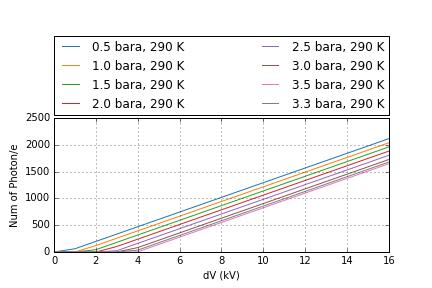
\includegraphics[width=0.9\textwidth]
  {Figures/Ch10/PhotonCreation_Naive.jpg}
  \caption{The number of photons created per electron between the anode grid and the gate grid. A $13 mm$ gap size is assumed.}
  \label{fig: Photon Creation Naive}
\end{figure}


\subsection{Light collection efficiency}
The light collection efficiency


\section{DAQ configuration, DAQ dead time and Required silence pre-trigger}




\section{Data processing}
%\begin{table}[!htbp]




\section{PMT single photo electron area calibration}  
\begin{center}
\begin{figure}[!htbp]
\begin{tabular}{|l|*{1}{c|}}\hline
\makebox[0.45\textwidth]{Top PMT}&\makebox[0.45\textwidth]{Bottom PMT}\\\hline\hline        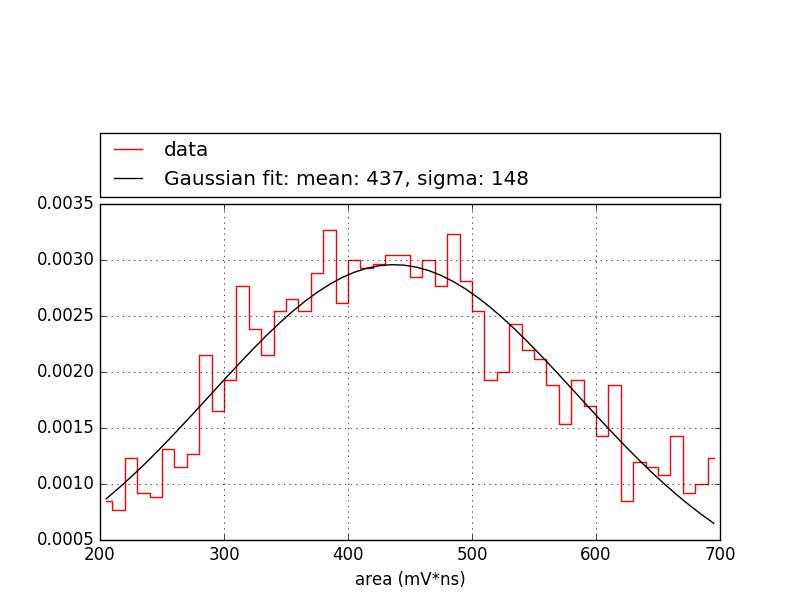
\includegraphics[width=0.45\textwidth]{Figures/Ch10/top_area.jpg} & 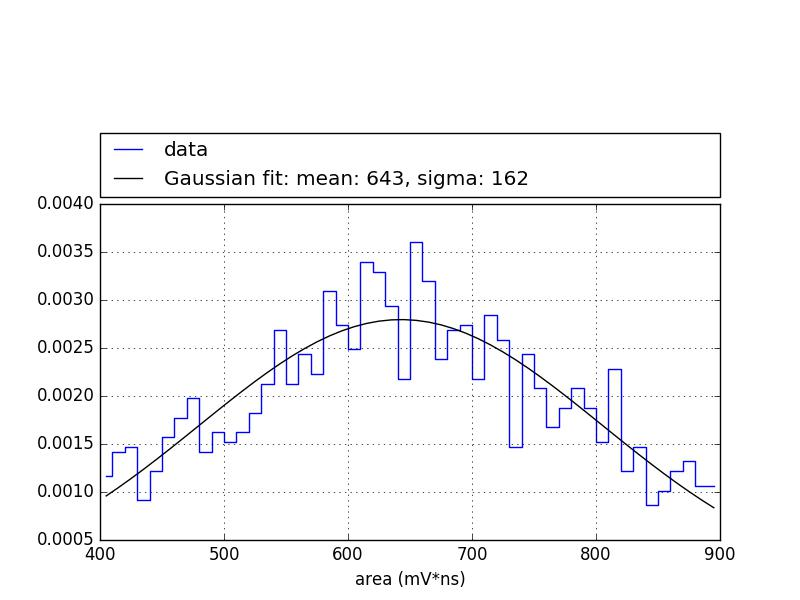
\includegraphics[width=0.45\textwidth]{Figures/Ch10/bot_area.jpg} \\ 
\multicolumn{1}{|m{0.45\textwidth}|}{}& \multicolumn{1}{m{0.45\textwidth}|}{}
\\\hline
    \end{tabular}
    \label{PMT calibration}
    \caption{PMT areas calibration.}
\end{figure}
\end{center}

\begin{table}[!htbp]
\begin{tabular}{|l||*{2}{c|}}\hline
&\makebox[7em]{Top PMT}&\makebox[7em]{Bottom PMT}\\\hline\hline
Single phe area ($mV \cdot ns$) &$437\pm148$&$643\pm162$\\\hline
\end{tabular}
\caption{PMT areas calibration.}
\end{table}



\section{Understanding of the events}
For clearly studying the grid wire electron emission events in the detector, understanding different types of background event rates events is necessary. To study this, first understanding the resources of these background and the general pulse shape of these events is necessary.\\
In this section, I will discuss about they different type of event happening in the detector. I will mainly focusing on discussing on the shape and the rate of these events and their impedance from these type of background events on the electron emission study.\\
The event class that we want to study are:\\
\begin{itemize}
\item Electron emission events from the grid wires.           
\item Electron emission events from the grid holding plates.
\end{itemize}
Electron emission events from the grid wires can be studied by the electroluminescence light from the emitted electrons. After the emitted electrons left the cathodic metallic grid, they would drift to the anodic grid by the Comlomb force between the two grids. During this process, these electrons will gain energy and accelerate from the Comlomb potential. The high speed electrons will lose their energy and create secondary particles through three processed. 1)exciting the gas atoms/molecules on their path, 2) ionizing the gas atoms/molecules on their path, or 3)or elastic scattering with the gas atoms/molecules on their path. The excited gas atoms/molecules would de-excite after a short amount of time and emit scintillation light photons. Usually these scintillation light photons were able to be re-absorded by the gas atoms/molecules because they have a similar energy compare to the exciting states of the gas atoms/molecules. However, for noble gas molecules, another type of deexcitation would happen. The excited noble gas molecule would find another noble gas molecule and found a two noble gas atom molecule excitation state. The two atom molecule, sometimes called a dimer, could also deexcite and emit a photon.\\ 
\begin{align}
M_2^* &\rightarrow M + M + \gamma.
\end{align}
However, this photon would have a different energy compare to the excited state of noble gas atom. Thus, this photon would propagated a further distance. The number of scintillation photons are mostly depending on the total Comlomb potential the electron gains from the trajectory and the energy loss by thermal inelastic scatterings. The former is a function of the potential difference between the two grids, when the latter is mostly a function of the length of the electron trajectory. The secondary scintillation light is found to have a linear dependence on the reduced field $E_s/N$ \cite{Monteiro2007}, where $E_s$ is the field strength in the scintillation light creation region and $N$ is the density of gas:
\begin{align}
&\frac{dL_s}{dx}=a \frac{E_s}{N} + b \\.
\end{align} 
The parameters $a$ and $b$ were found to be
\begin{align}
a &= 0.137(2)\frac{ph}{e\cdot V}, \\
b &= -4.7(1) \times 10^{-18} \frac{ph}{e} \frac{cm^2}{atom}.
\end{align}
\\
Thus, with counting the scintillation photons over time, a grid emission event can be distinguished from the other type of events that occurred in the detector, which would be discussed late in this paragraph.\\ 
The excited dimer molecules can be separated to two types, the singlet state and triplet state. The singlet state, written as $^1\sigma_u^+$, $0_u^+$, the triplet state, written as $^3\sigma_u^+$, $1_u^+$,  are known to be created from a three-body deconstruction of noble gas atom excited state $^2P_{1/2}$ state and $^2P_{3/2}$ state.  \\
\begin{align}
M + M + M^* &\rightarrow M + M_2^* +E_k\\
\end{align}
Because the creation process is a three body reaction, the creation rate of the these two states have strong dependence on the gas density of atoms. The decay time of both of these two states have a dependence on the gas density. \cite{Keto1974}. Some other materials also show that the decay time is very different between liquid noble gas and very dense noble gas. \\
The decay time for the singlet state and the triplet state in liquid xenon are $4.3 \pm 0.6 ns$ and $22.0 \pm 2.0 ns$ \cite{Hitachi1983}. And for dense xenon, $2.7$ to $32 atm$, the decay time for singlet states varies from $15 \pm 3 ns$ to $5.5 \pm 1 ns$. The decay time for triplet state is $96 \pm 5 ns$ in the same pressure range.\\
The decay time for the singlet state and the triplet state in liquid argon are $7.0 \pm 1.0 ns$ and $1.6 \pm 0.1 \mu s$. And for dense argon, the decay time for singlet states is $4.20 \pm 0.13 ns$. The decay time for triplet state is $3.2 \pm 0.3 \mu s$\\ 
The ionization of gas atoms/molecules happens along with scintillation process. When the incident electron exceed the ionization energy of the gas atoms/molecules, their is a chance that an inner shell electron would leave the gas atoms/molecules. The cross-section of ionization are excitation probabilities as a function of incidence electron are shown in \ref{fig: xenon exc ion}. The ionization probability increase as the energy of incident electron. In a higher electric field space or a lower gas density situation, the average energy an electron can gain between each collision is higher. Thus, ionization are more commonly seen in these situation. \\
A critical threshold electric field density is where ionization become important (>$1\%$) for gas. During our operation, the electric field between the two grids are much smaller than this critical threshold, while the electric field on the surface of the grid is sometimes higher than this critical threshold. Very few ionization events happens in the main scintillation region, and most of the ionization happens around the grid wires. This is consistent with what we saw in data.\\
The creation of excitation photons and ionization atoms and secondary electrons are also studied with simulation software. The    
\\
The backgrounds in the detector can be separated to three categories: noise, external and internal particle events and others. These background events are:\\
\begin{itemize}
\item Electronic noise
	Electronic noise is the irreducible
	\subitem Electronic noise type 1: photomultiplier tube(PMT) noise
    Photomultiplier tube noise is coming from the thermeonic emission  
    \subitem Electronic noise type 2: building power supply noise
\item External and internal particles	 
	\subitem Radiation from the detector component
	\subitem High energy muon from cosmic rays
	\subitem High energy external gamma 
\item Other trouble:
	\subitem photomultiplier tube(PMT) baseline shifting
    \subitem photomultiplier after pulsing
    \subitem two photo electron accidental false coincidence in two photomultiplier tubes(PMT)(dark current)
    \subitem discharging from the cable feed through and connectors.
    \subitem delayed light from big events (Polytetrafluoroethylene(PTFE) fluorescence)
\end{itemize}


External and internal particles in the gaseous medium will deposit their energy on their trajectory.
\begin{itemize}


\item S1 light: initial scintillation light from direct scintillation of gas molecules and immediate recombination of ionized gas molecules and electrons
	\subitem S1 inside the scintillation region (between the two grids)
	\subitem S1 outside the scintillation region , the anodic biased grid side
    \subitem S1 outside the scintillation region , the cathode biased grid side
\item Gas S2 light: scintillation light created from electrons outside scintillation region landing on the anodic bias grid
\item S2 light: scintillation light created from electrons passing the scintillation region
\end{itemize} 

S1 event: 

\begin{center}
\begin{figure}[!htbp]
  \centering
  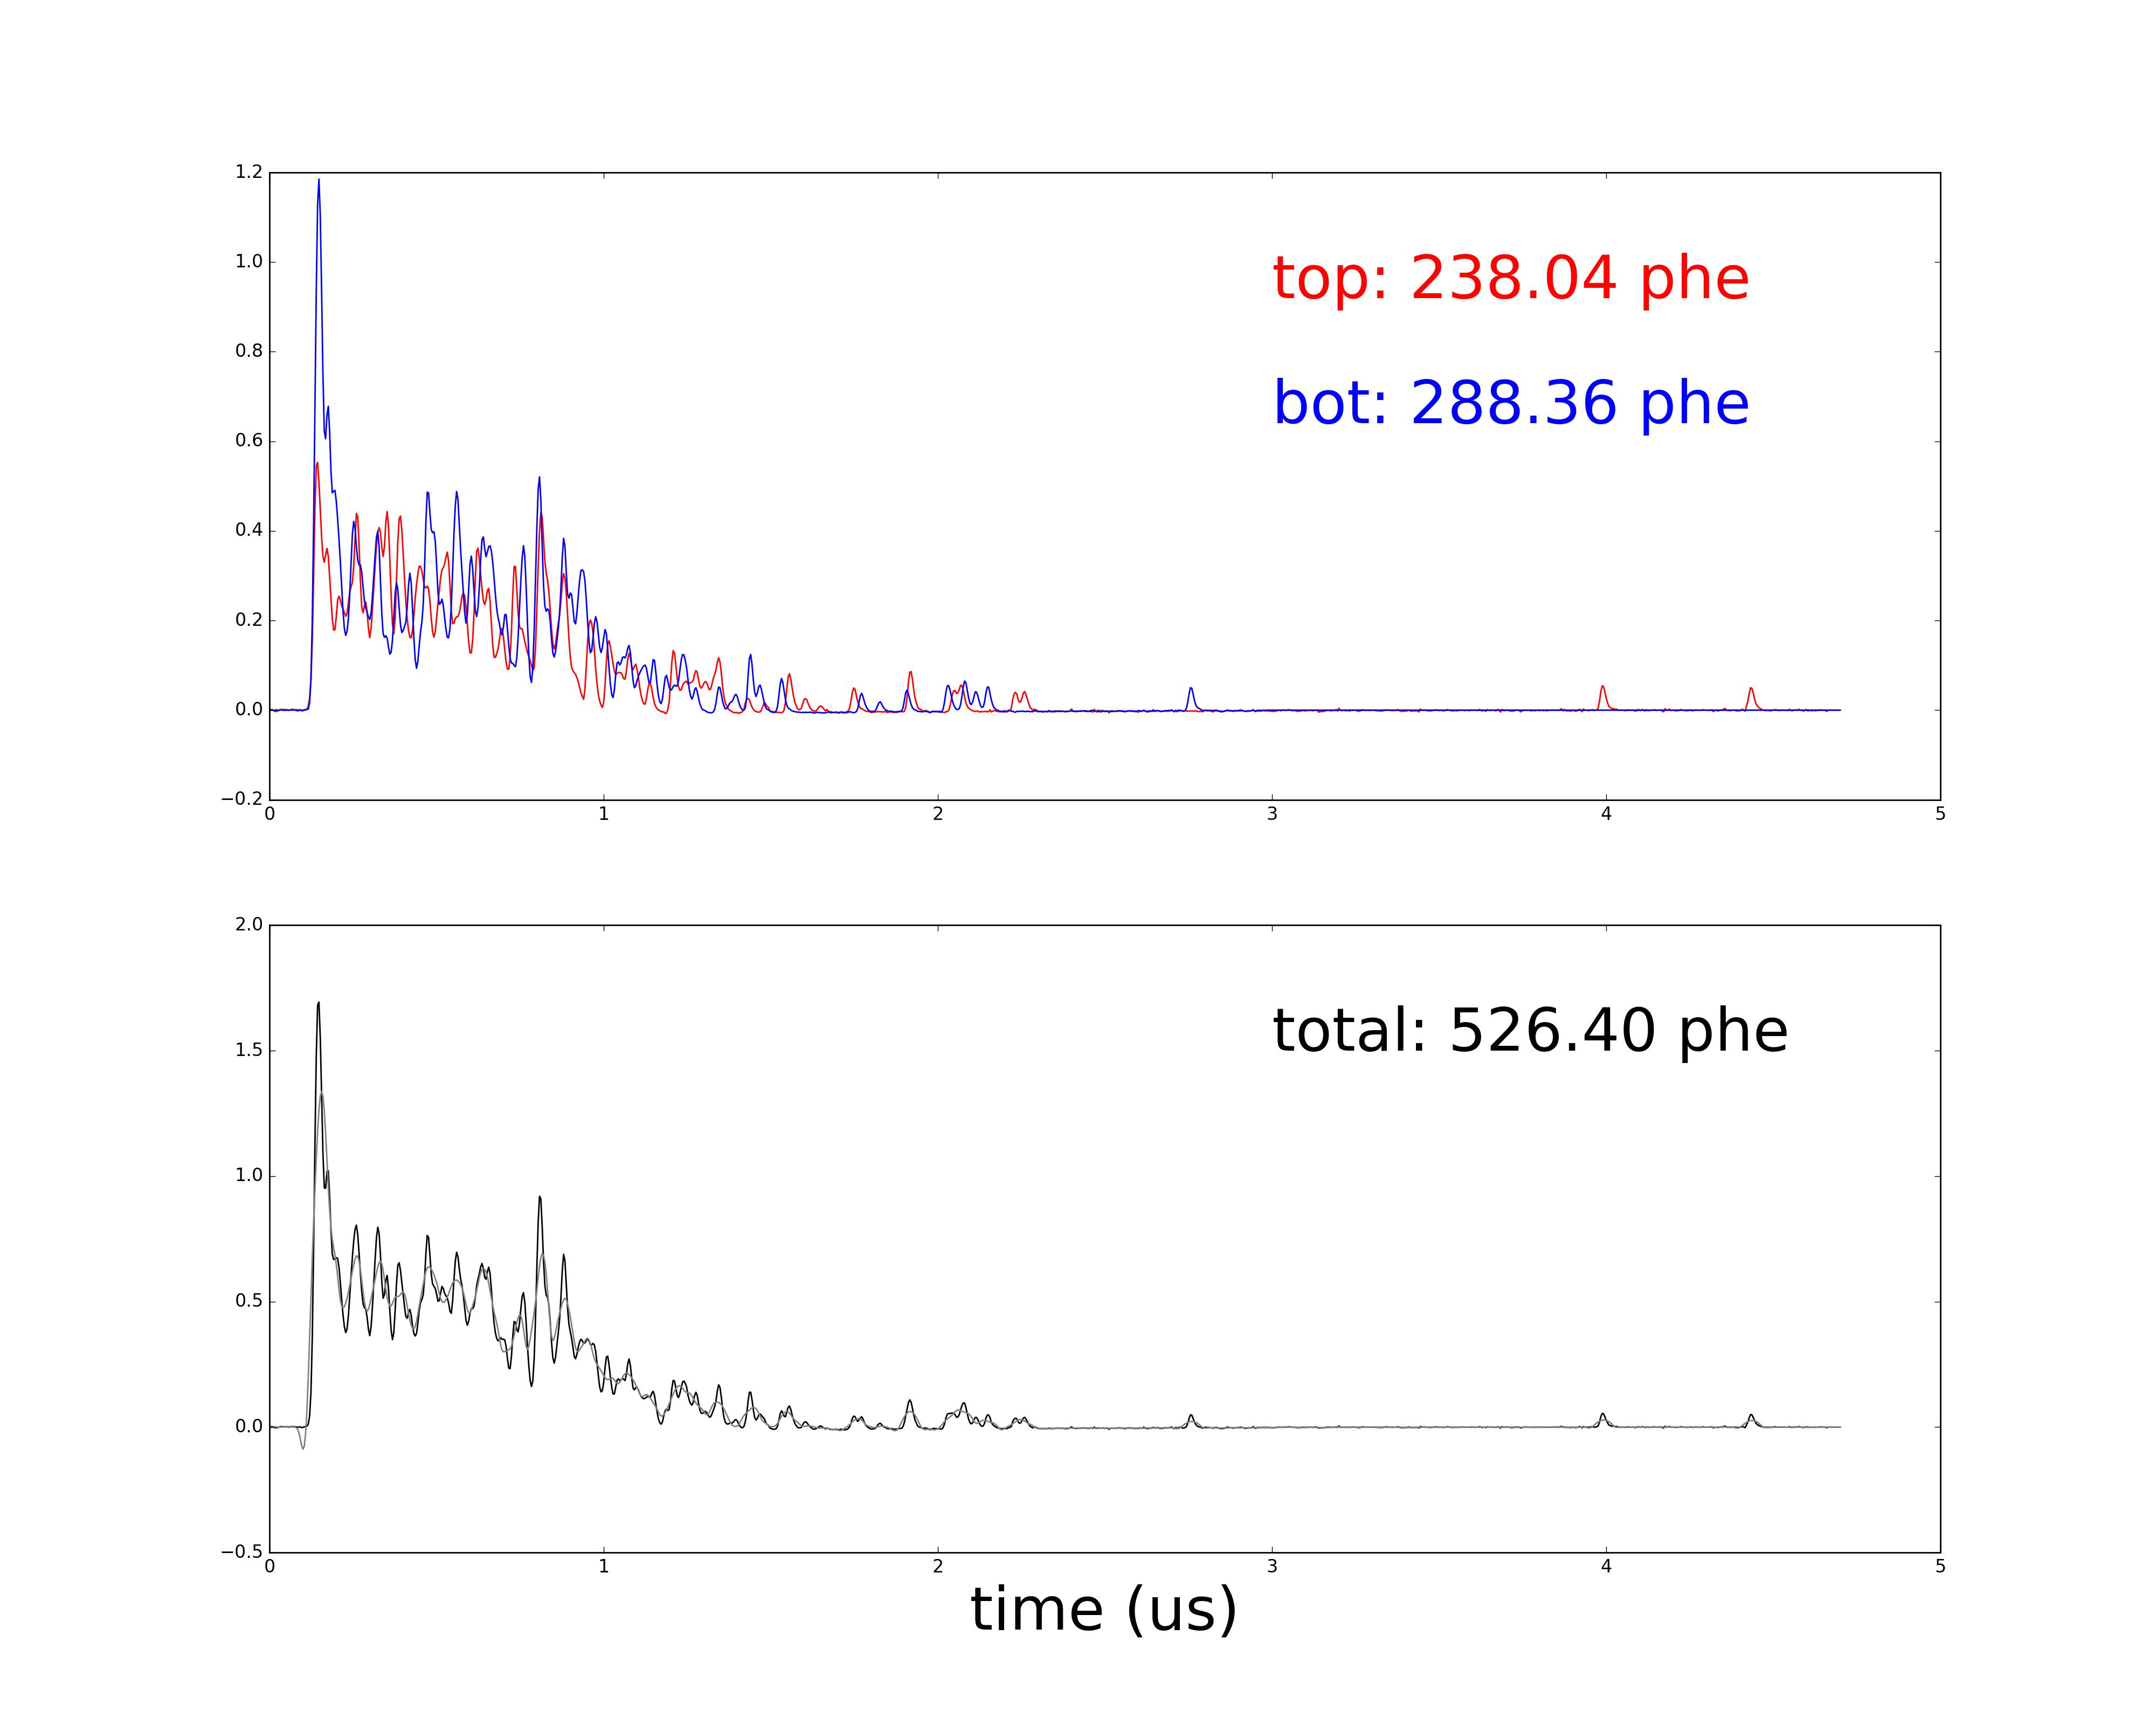
\includegraphics[width=0.8\textwidth,clip,trim={0 0 0 0}]
  {Figures/Ch10/SampleWaveforms/_64767_a_+6_0_g_-6_0_Cut33_big_pulse_PlotCoinWaveforms_42_.jpg}
  \caption{An external electron event: S1 event(first $100 ns$) occurred inside the scintillation region and S2 event(rest), light created by electrons passing through the scintillation region. Red line is top PMT. Blue line is bottom PMT. Black line is the sum of the top and bottom PMTs. }
  \label{fig: external electron}
\end{figure}
\end{center}

\begin{center}
\begin{figure}[!htbp]
  \centering
  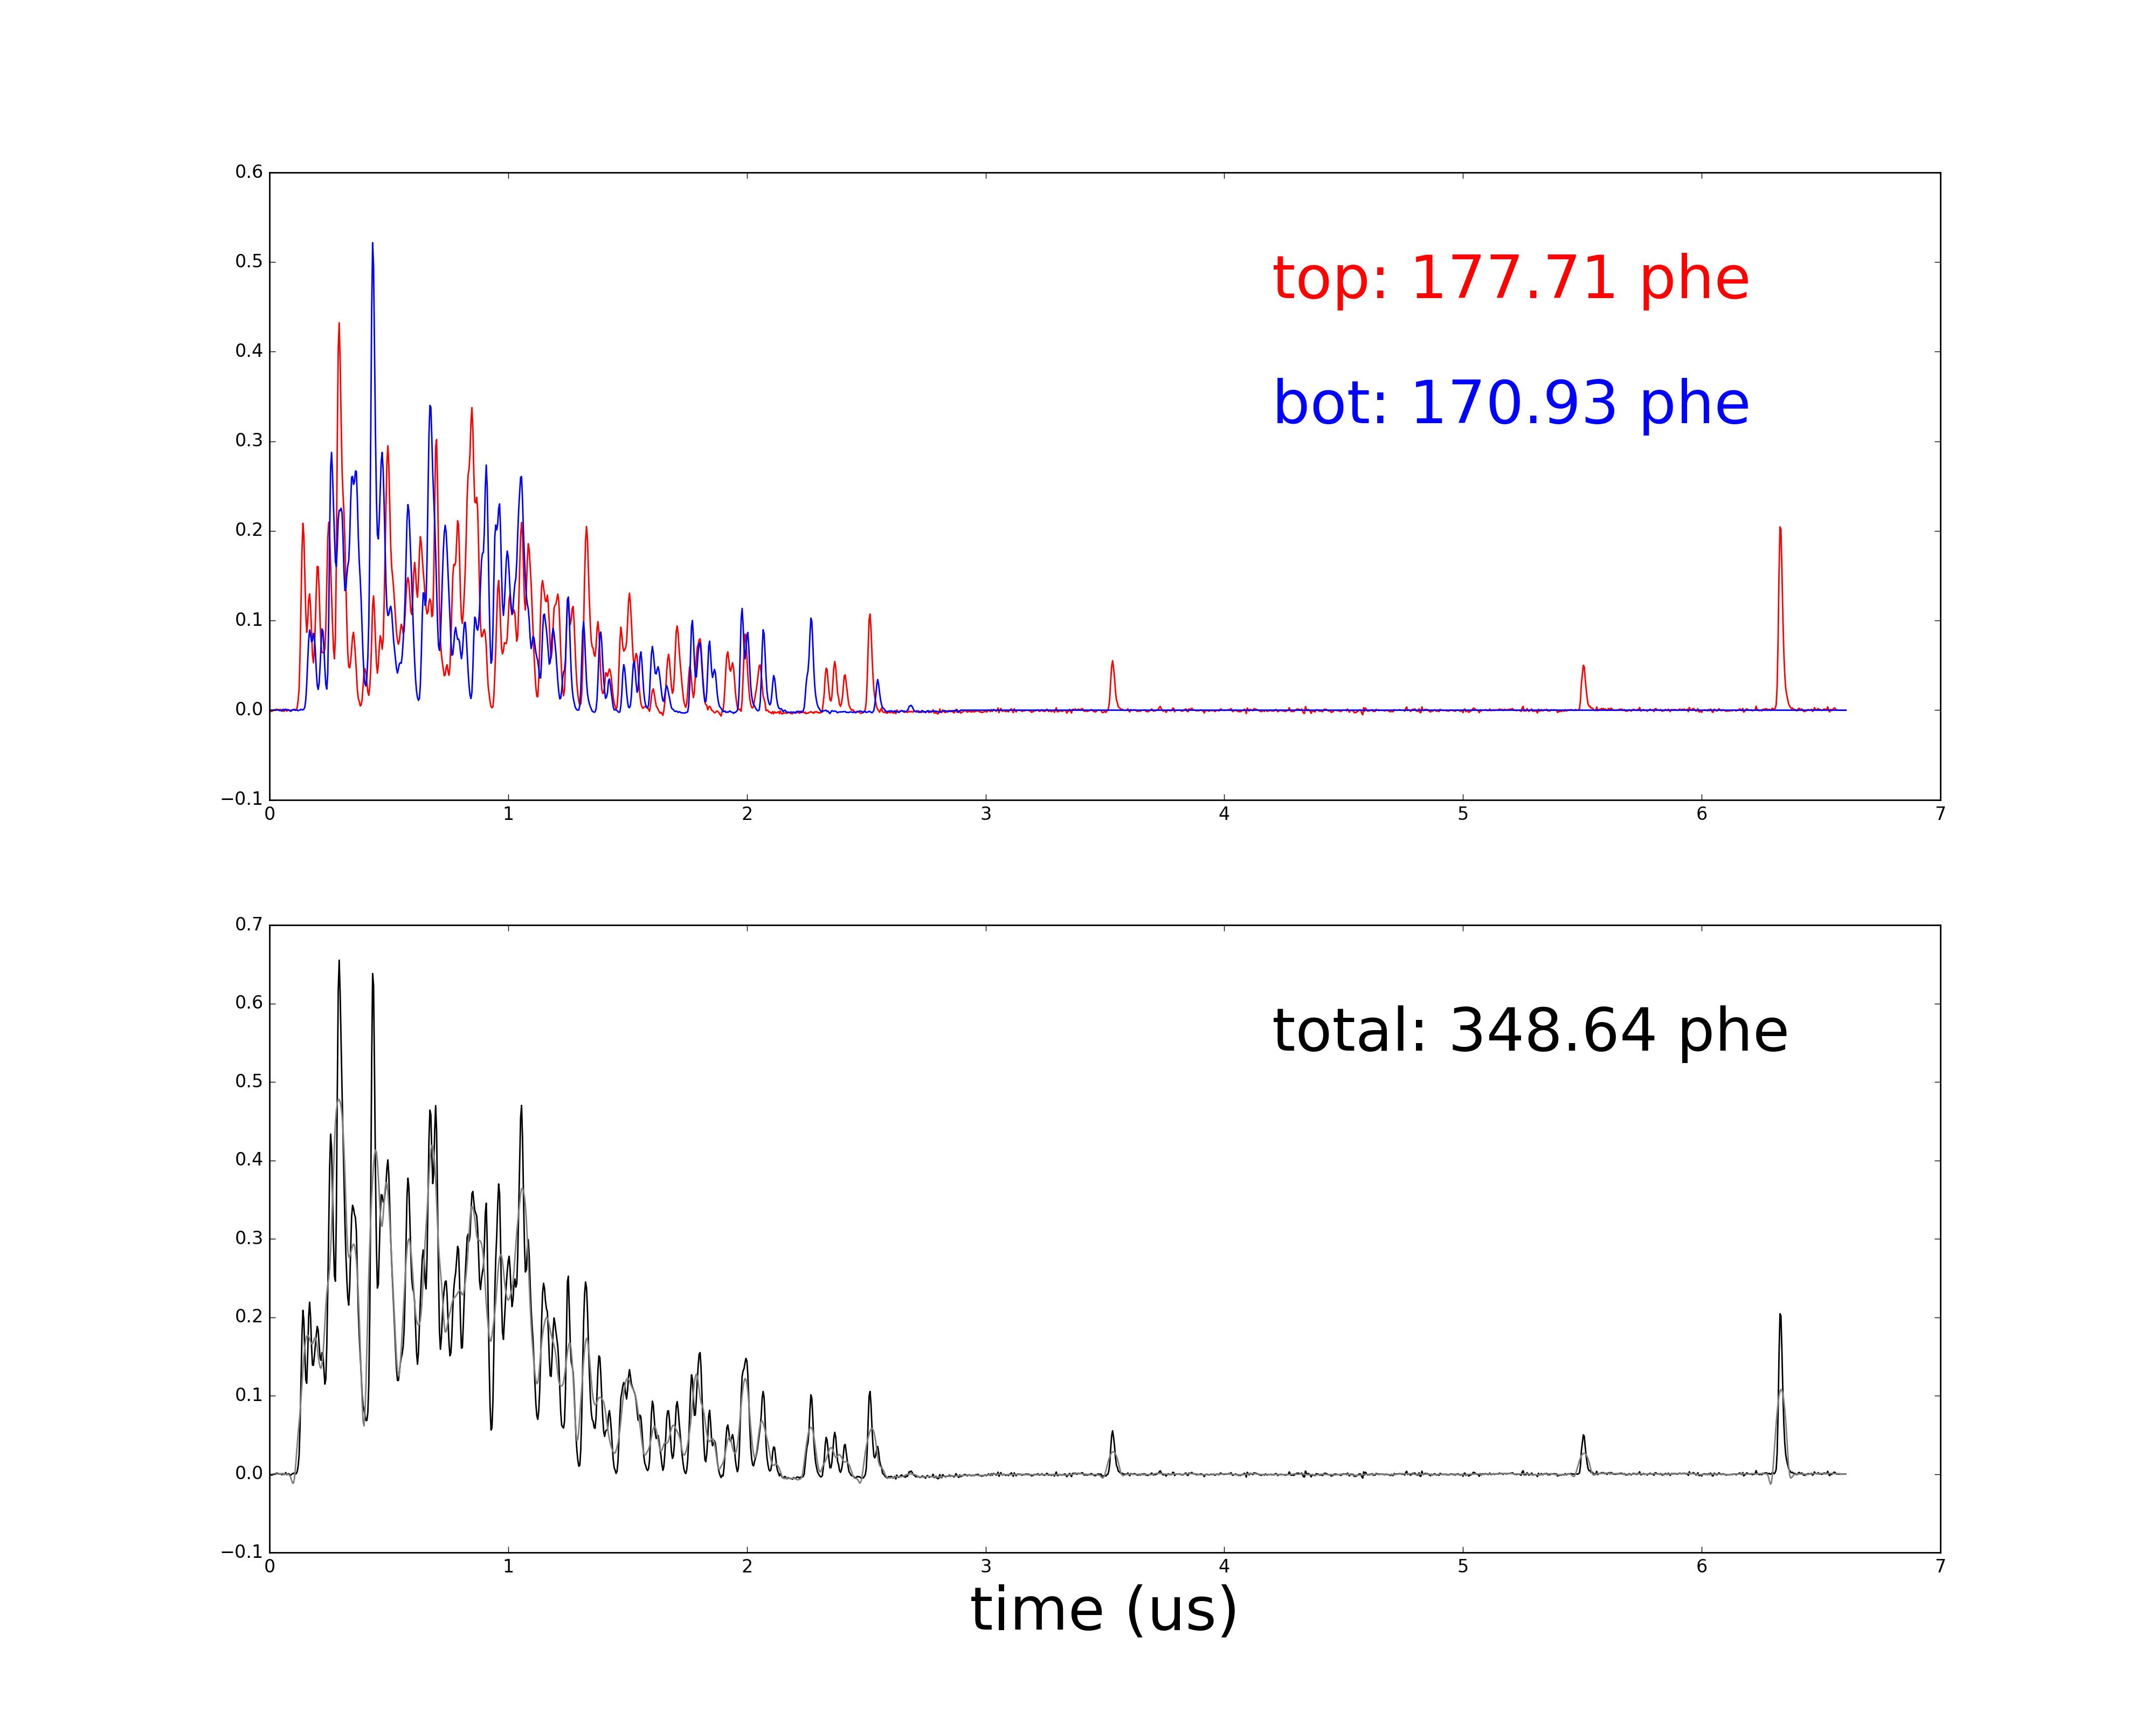
\includegraphics[width=0.8\textwidth,clip,trim={0 0 0 0}]
  {Figures/Ch10/SampleWaveforms/_64767_a_+6_0_g_-6_0_Cut33_big_pulse_PlotCoinWaveforms_1_.jpg}
  \caption{An Muon event: light created by electrons ionized by high energy muon in the scintillation region. Red line is top PMT. Blue line is bottom PMT. Black line is the sum of the top and bottom PMTs.}
  \label{fig: Muon}
\end{figure}
\end{center}

\begin{center}
\begin{figure}[!htbp]
  \centering
  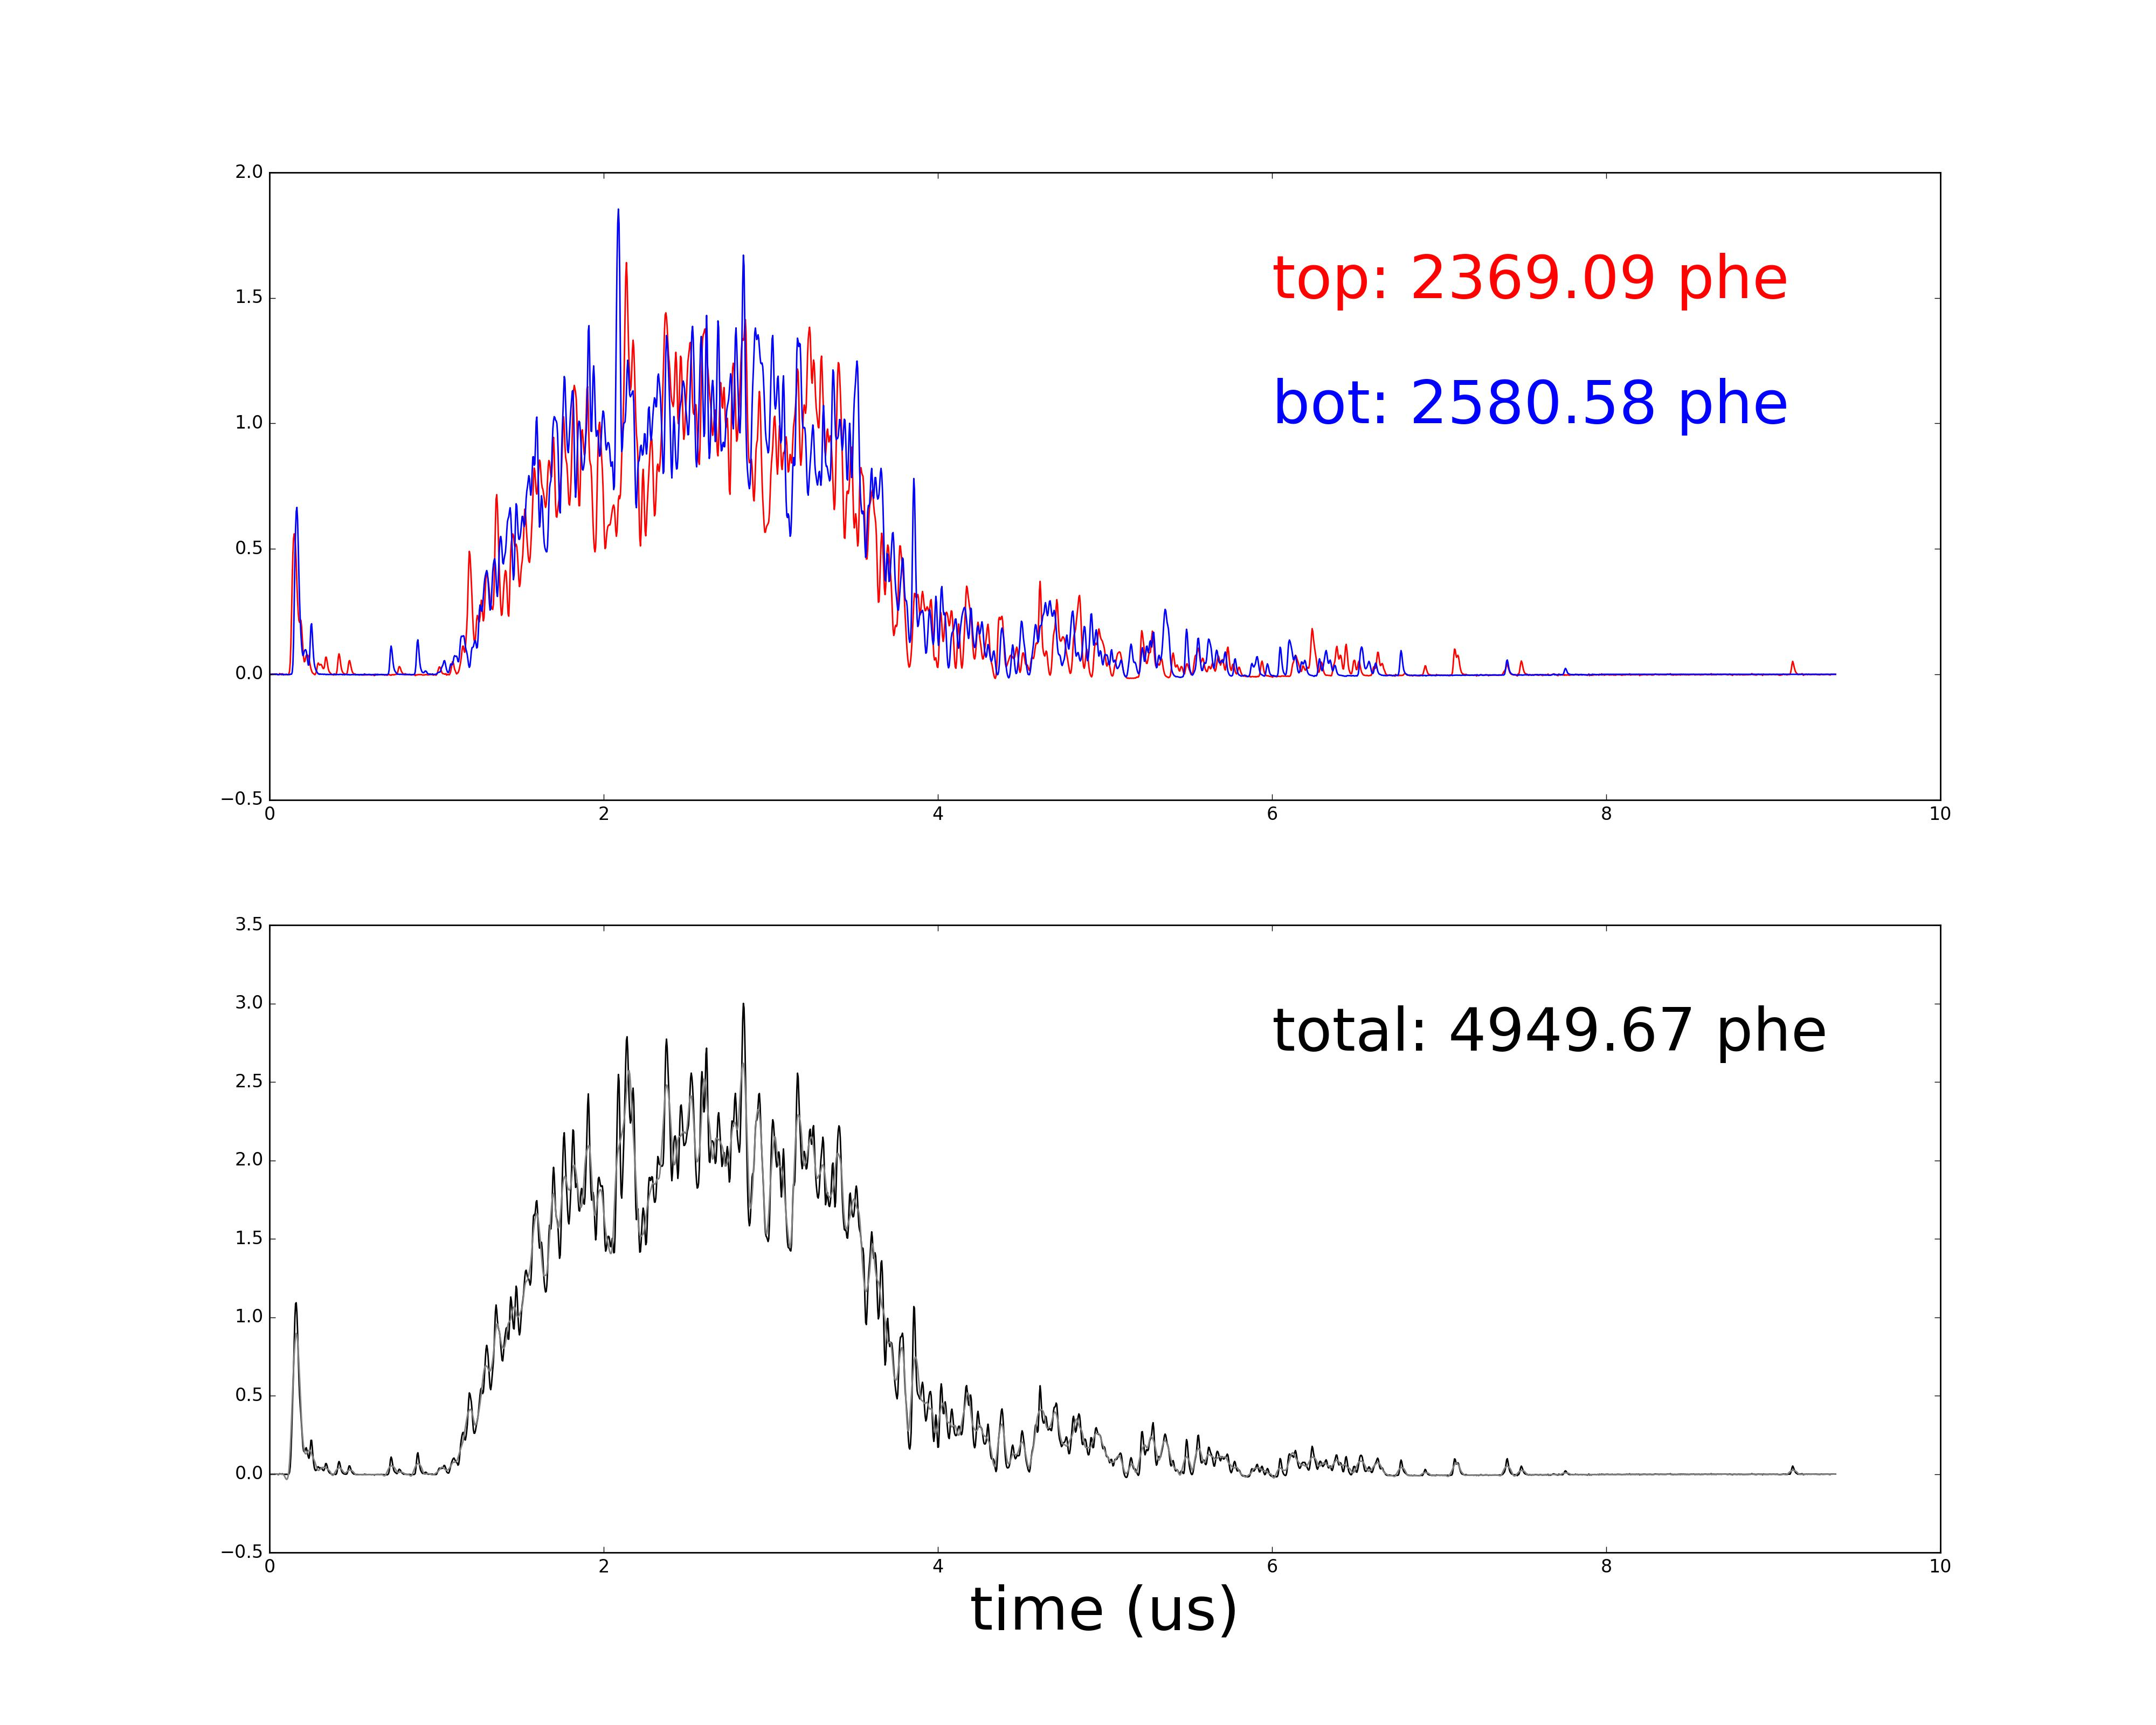
\includegraphics[width=0.8\textwidth,clip,trim={0 0 0 0}]
  {Figures/Ch10/SampleWaveforms/_64767_a_+6_0_g_-6_0_Cut33_big_pulse_PlotCoinWaveforms_84_.jpg}
  \caption{An S1 S2 event: S1 event(first $300 ns$) occurred outside the scintillation region and S2 event(rest), light created by electrons passing through the scintillation region. Red line is top PMT. Blue line is bottom PMT. Black line is the sum of the top and bottom PMTs. }
  \label{fig: S1 S2}
\end{figure}
\end{center}

\begin{center}
\begin{figure}[!htbp]
  \centering
  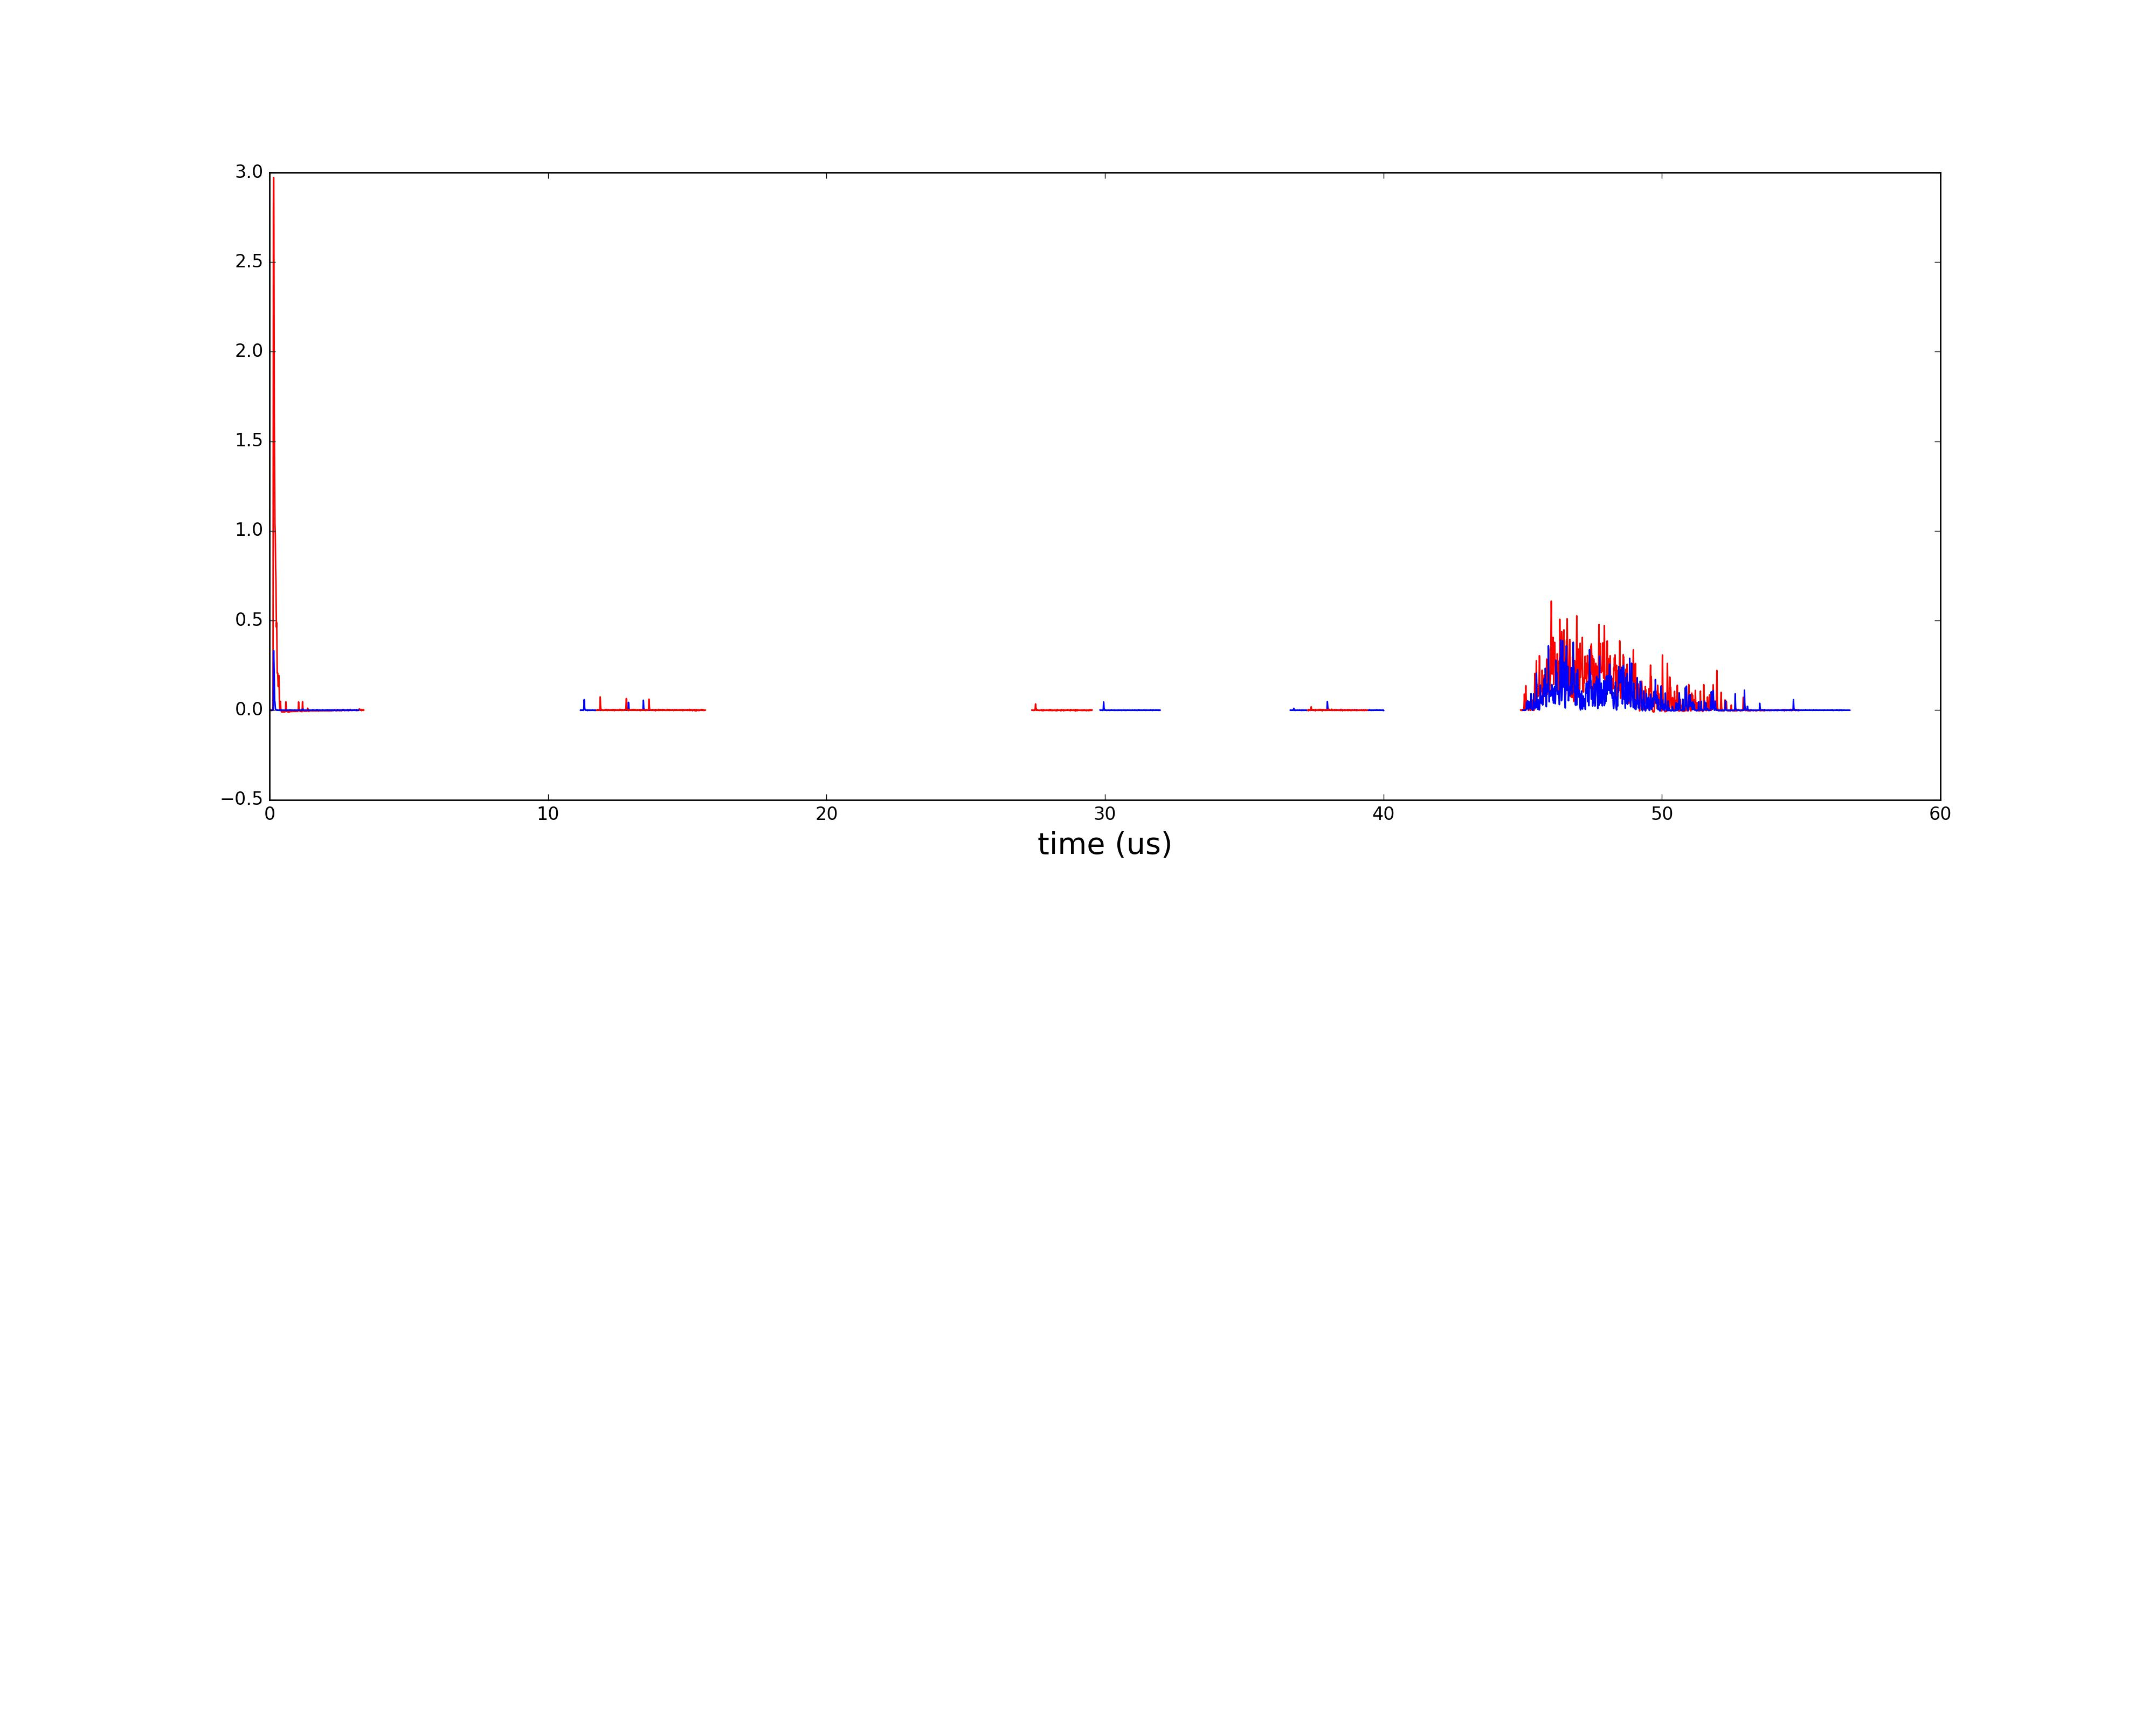
\includegraphics[width=0.8\textwidth,clip,trim={0 600 0 0}]
  {Figures/Ch10/SampleWaveforms/_64767_a_+6_0_g_-6_0_PlotCoinWaveforms_Plotid38183_.jpg}
  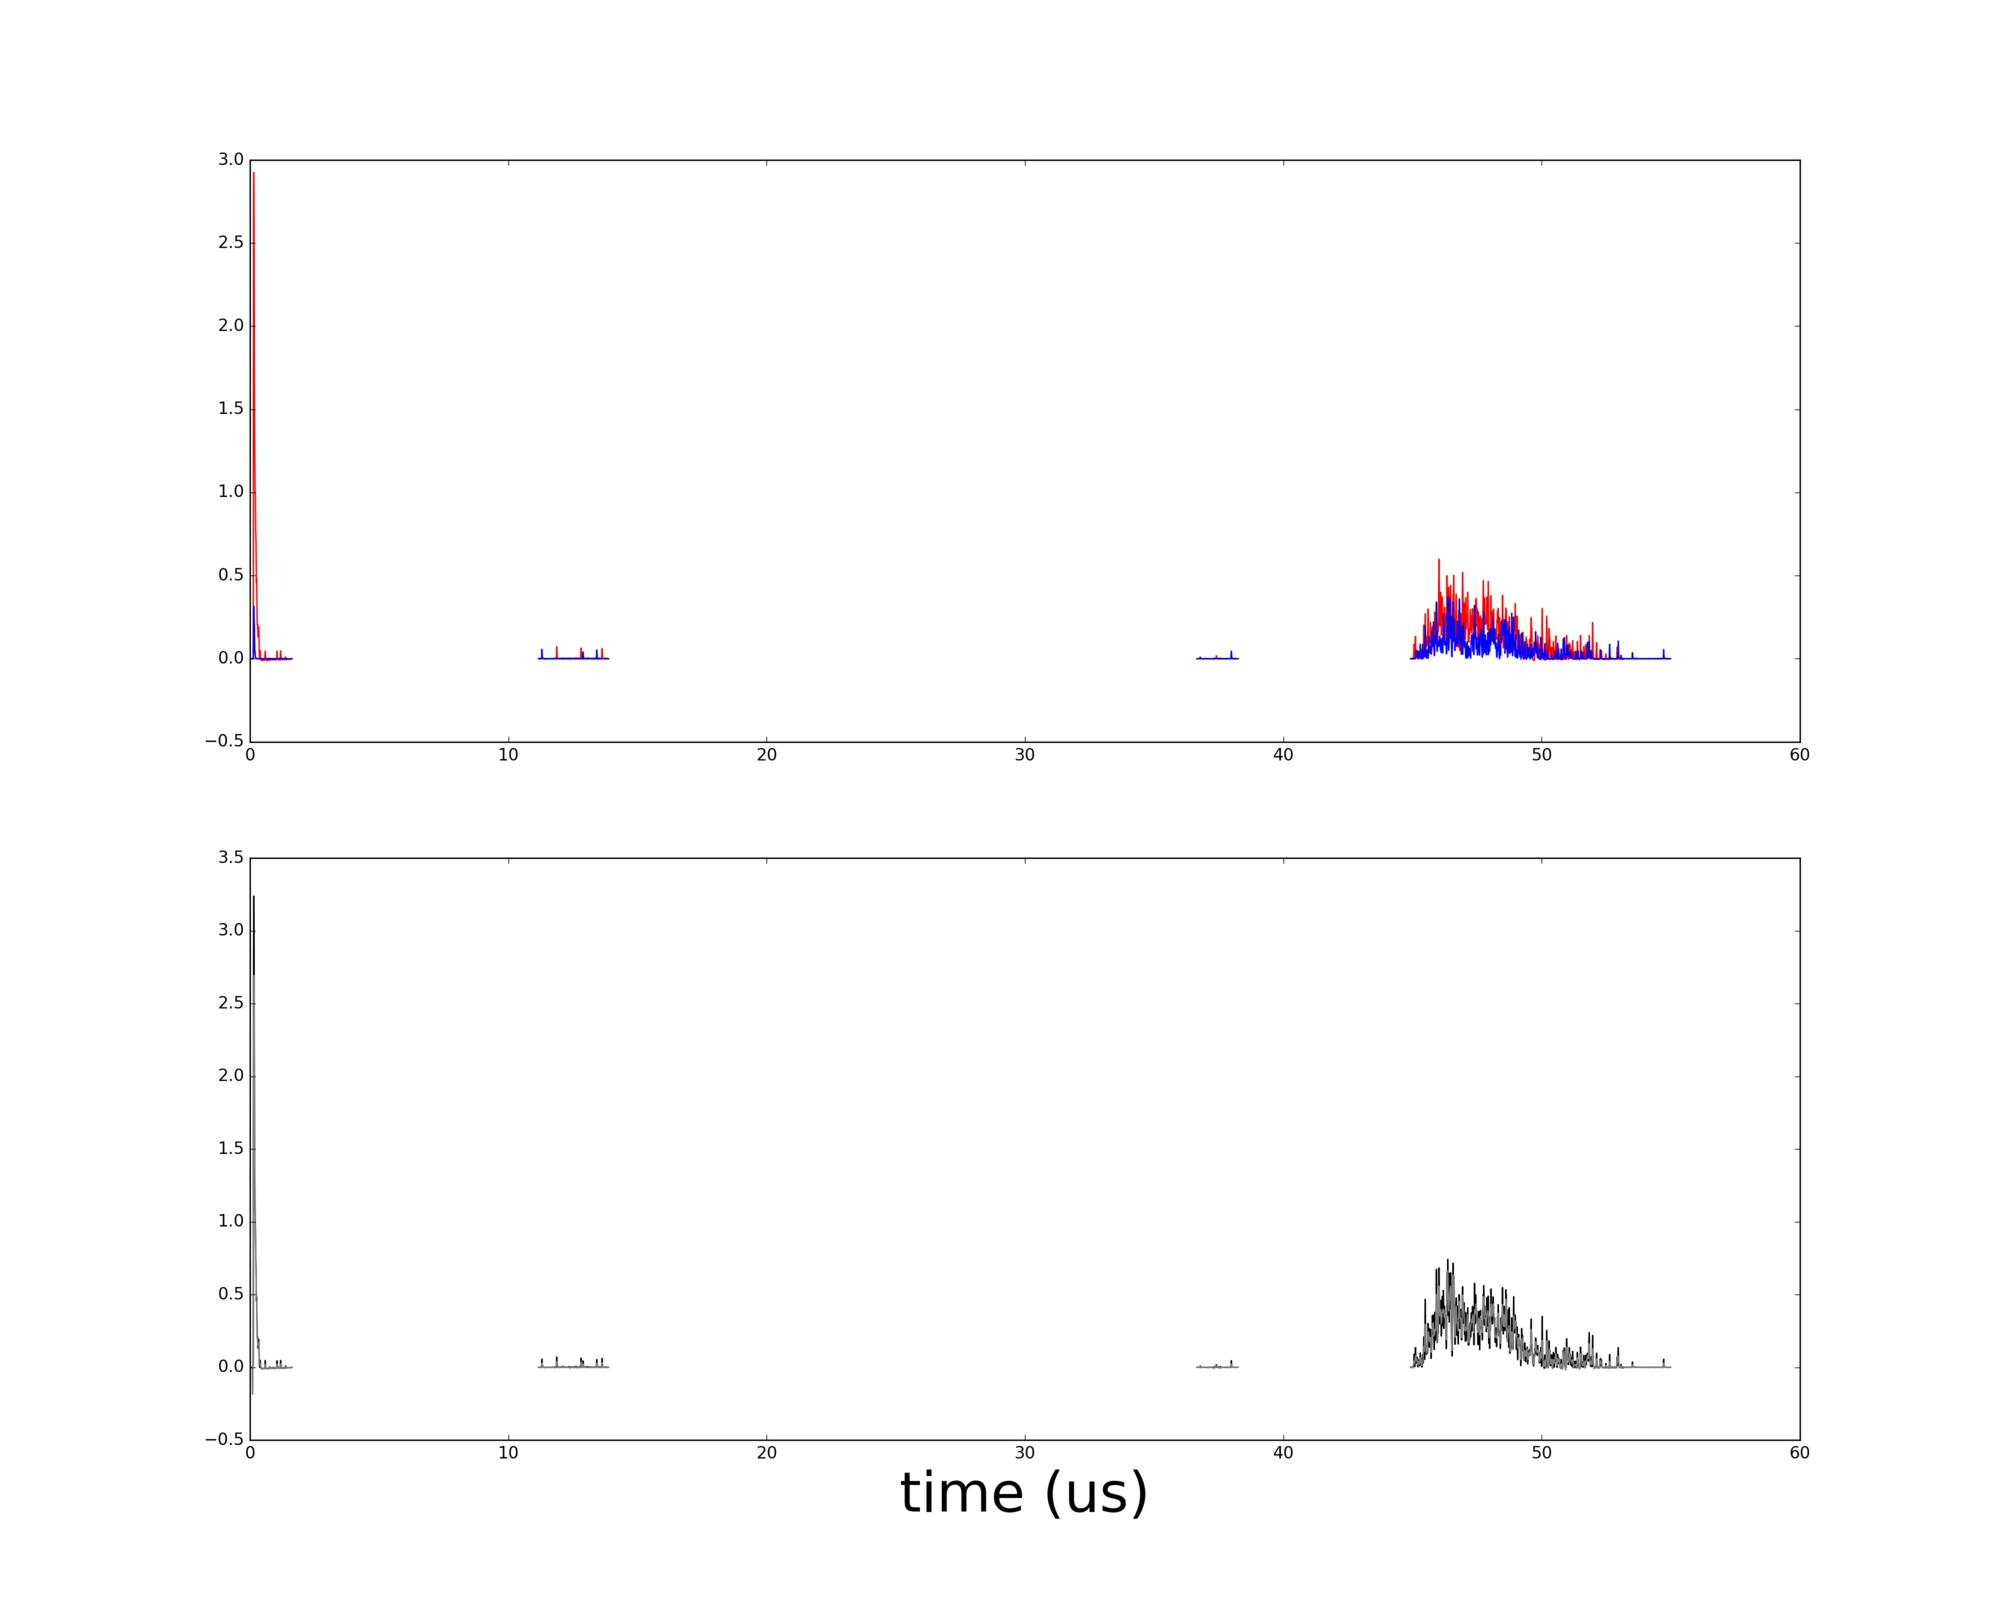
\includegraphics[width=0.8\textwidth,clip,trim={0 0 0 0}]
  {Figures/Ch10/SampleWaveforms/4.jpg}
  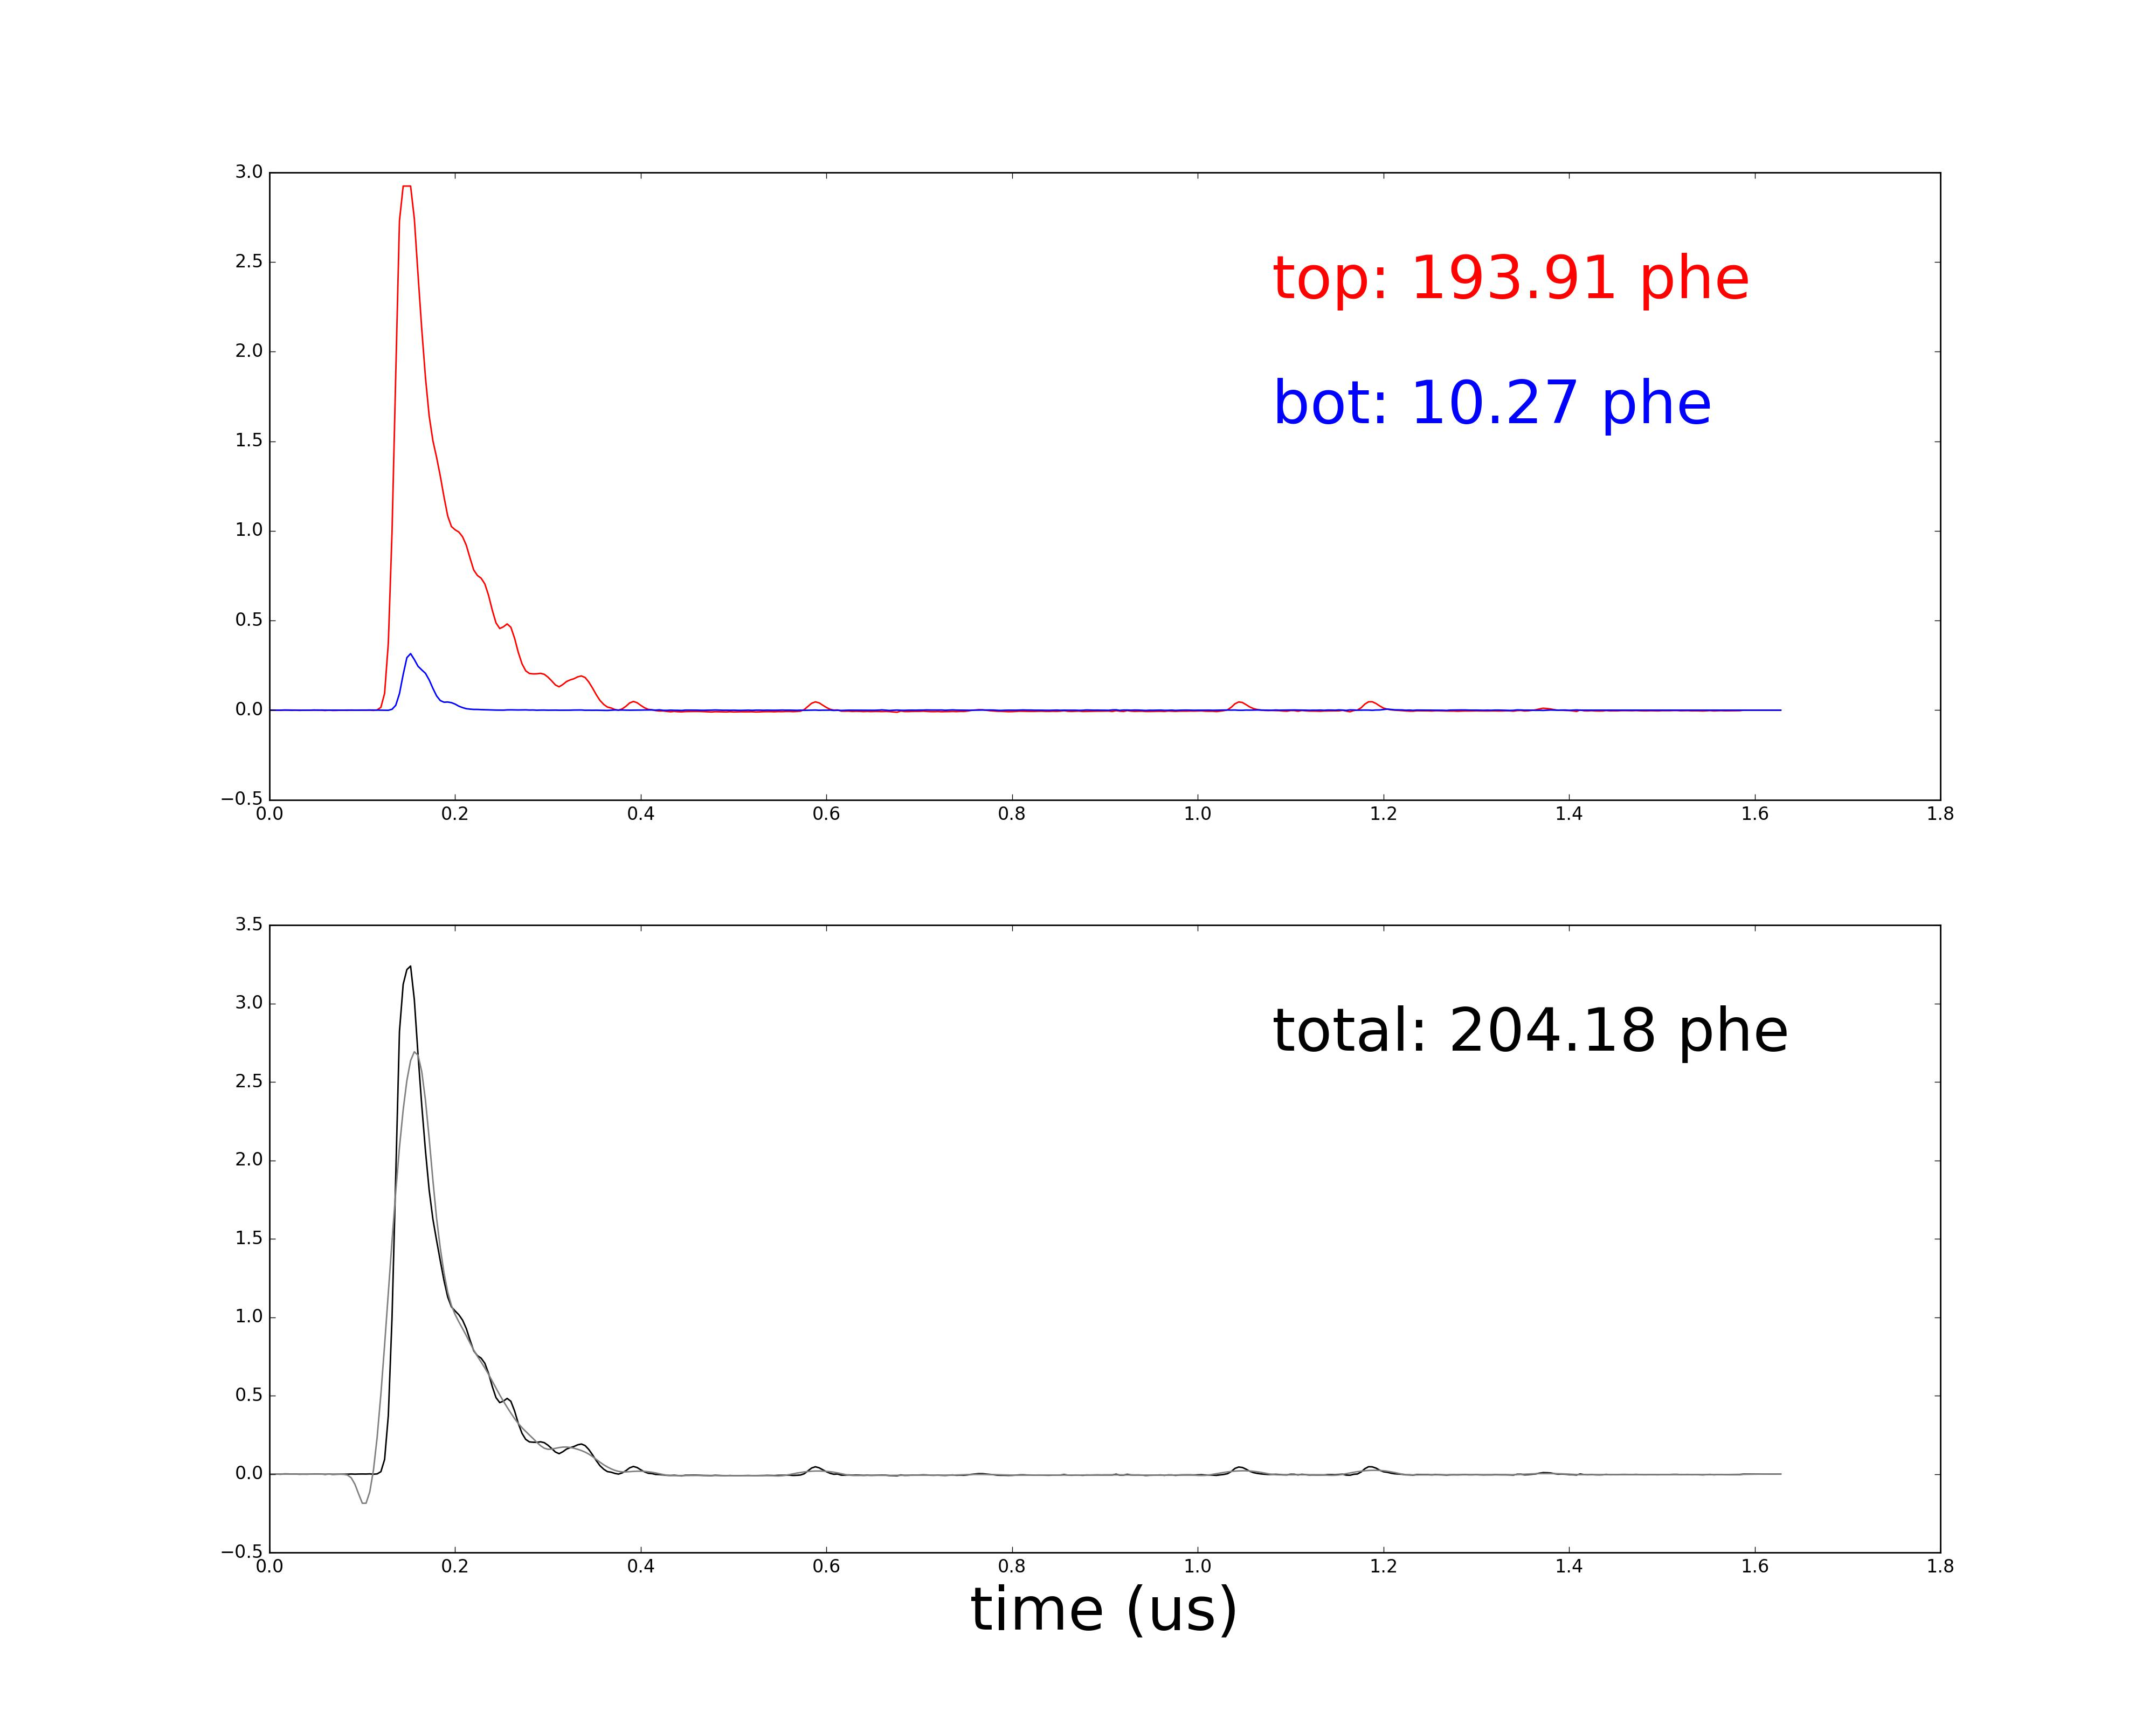
\includegraphics[width=0.35\textwidth,clip,trim={0 600 0 0}]
  {Figures/Ch10/SampleWaveforms/_64767_a_+6_0_g_-6_0_PlotCoinWaveforms_Plotid3179_.jpg}
  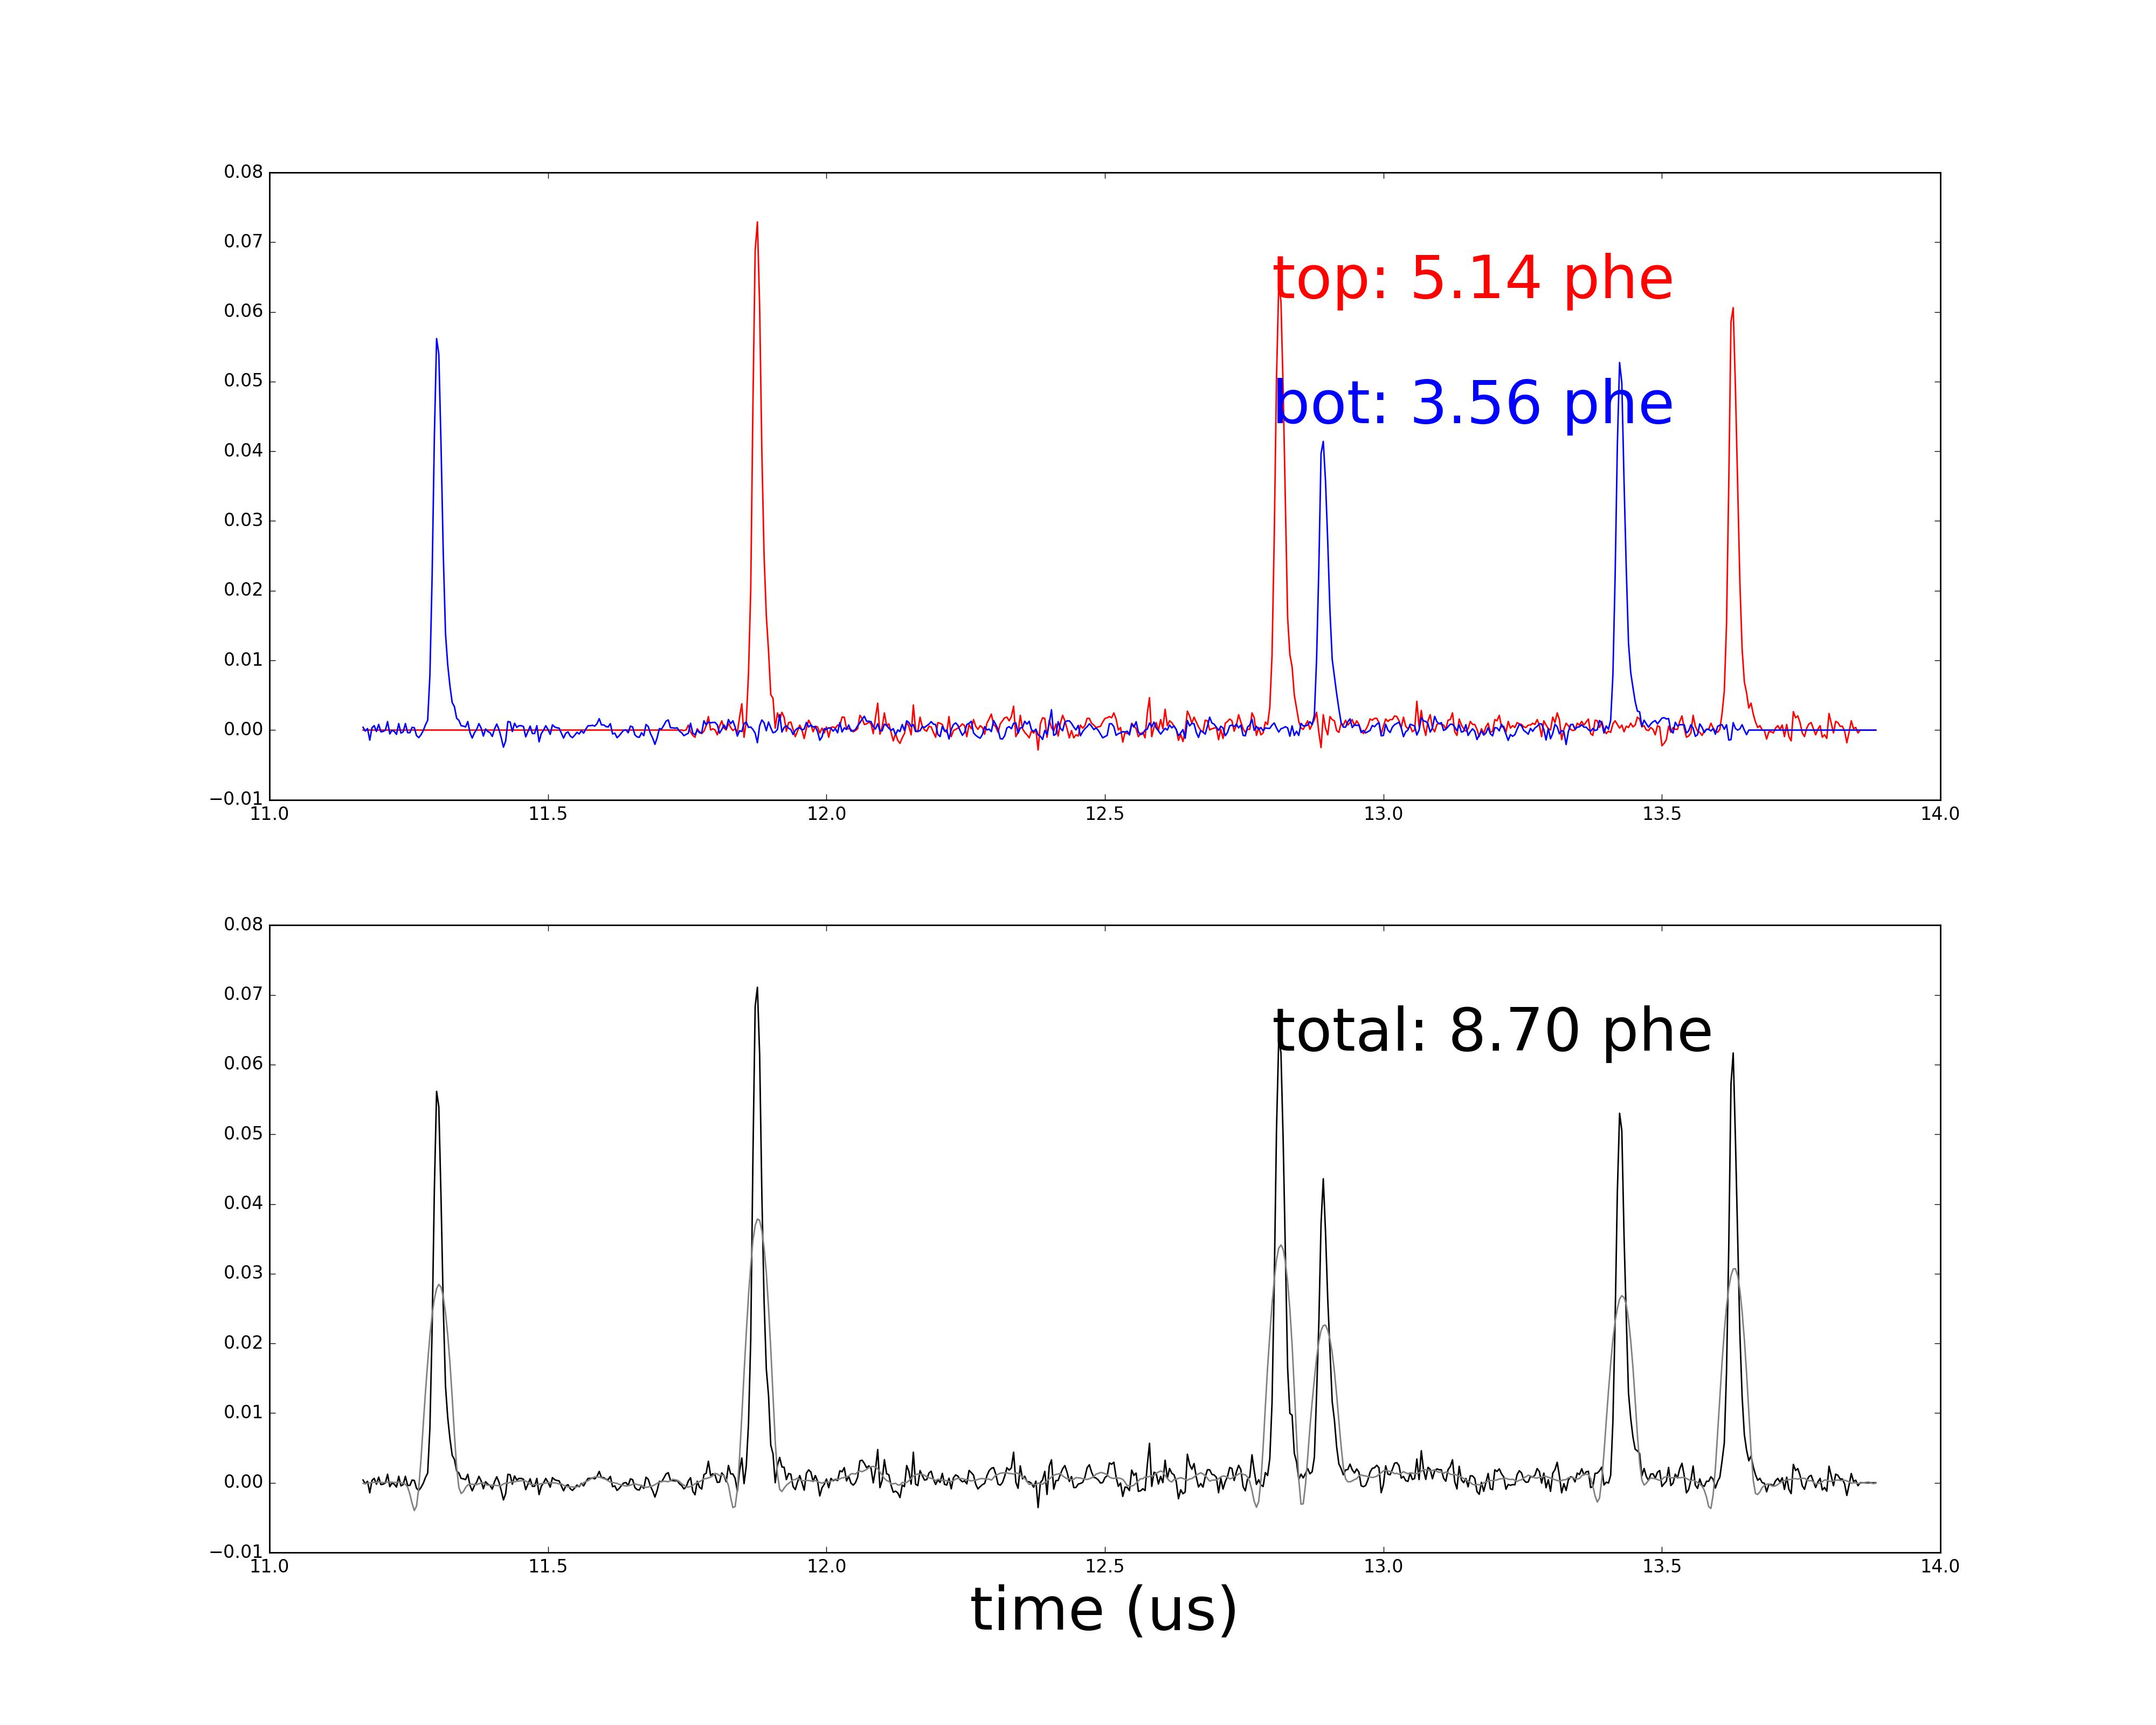
\includegraphics[width=0.35\textwidth,clip,trim={0 600 0 0}]
  {Figures/Ch10/SampleWaveforms/_64767_a_+6_0_g_-6_0_PlotCoinWaveforms_Plotid3180_.jpg}
  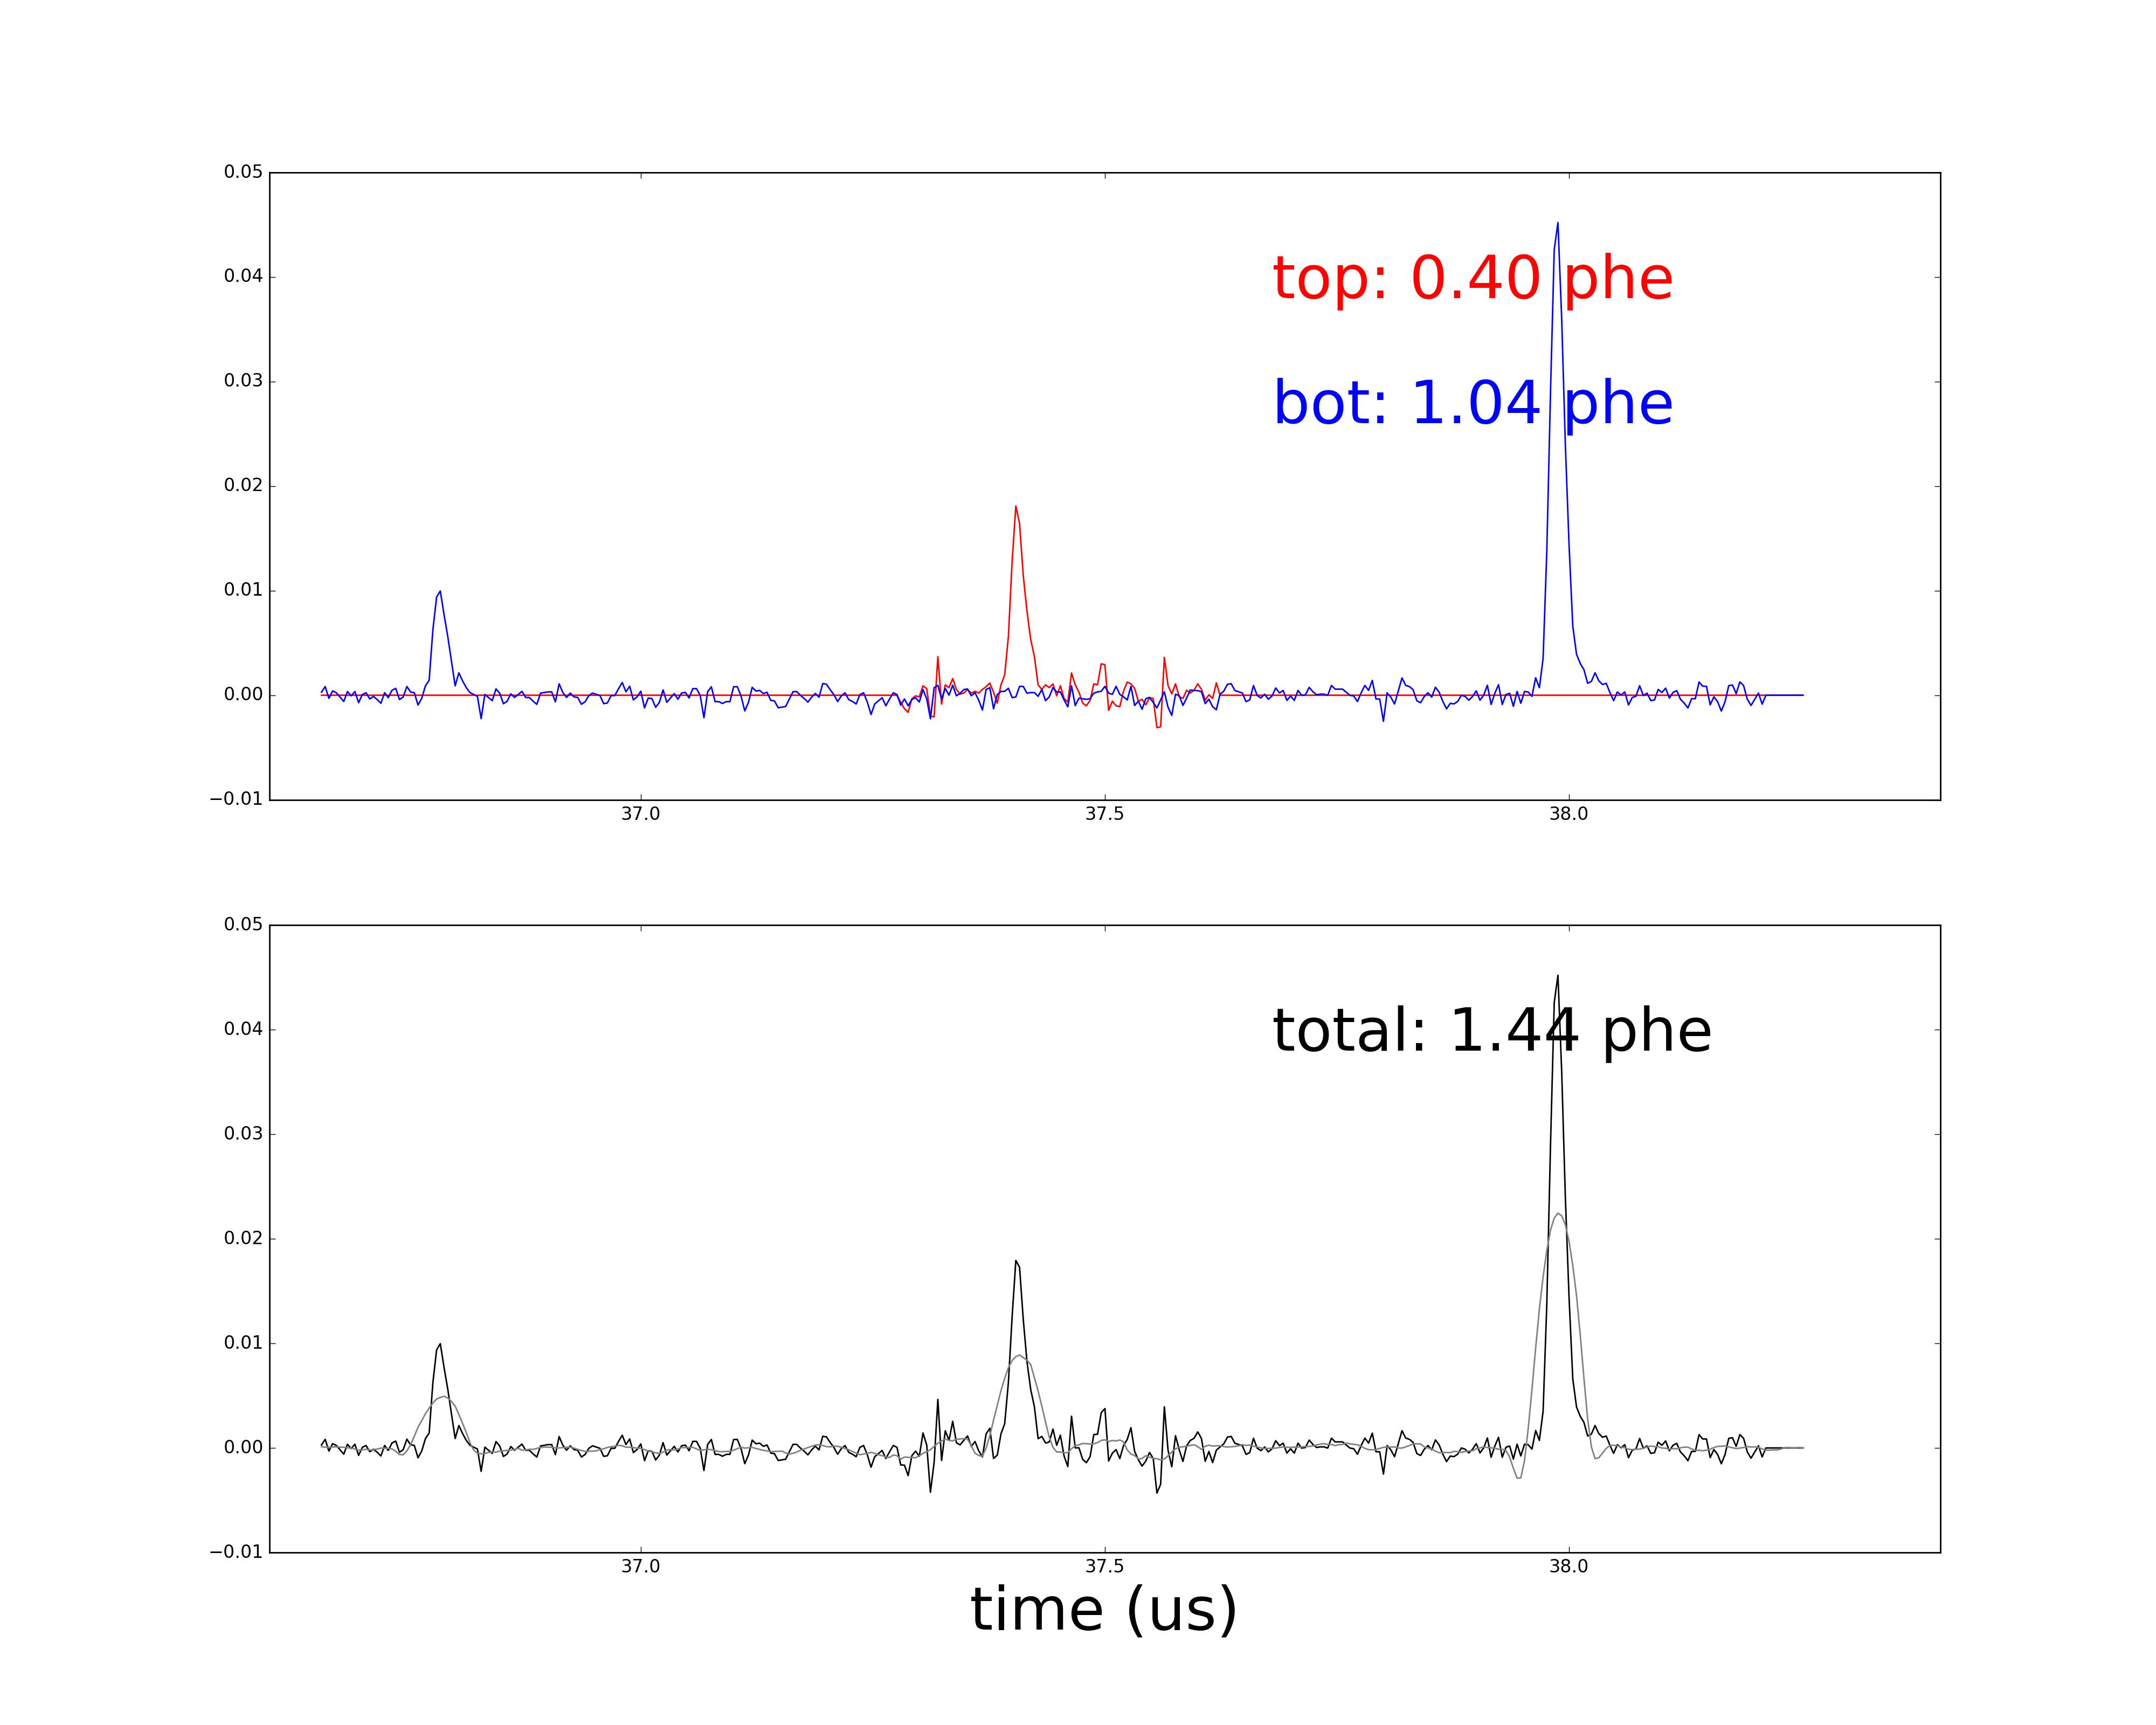
\includegraphics[width=0.35\textwidth,clip,trim={0 600 0 0}]
  {Figures/Ch10/SampleWaveforms/_64767_a_+6_0_g_-6_0_PlotCoinWaveforms_Plotid3181_.jpg}
  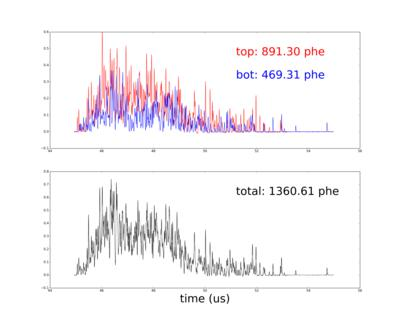
\includegraphics[width=0.35\textwidth,clip,trim={0 600 0 0}]
  {Figures/Ch10/SampleWaveforms/3182.jpg}
  \caption{A gas event: S1 event(first pulse) occurred outside the scintillation region and gas S2(else) occurred when the electrons created outside scintillation region landing on anodic grids. Top: all pulses recorded. Middle: coincidence pulses in top and bottom channels. Bottom: separate coincidence pulses. Red line is top PMT. Blue line is bottom PMT. Black line is the sum of the top and bottom PMTs. }
  \label{fig: S1 gas S2}
\end{figure}
\end{center}


\begin{center}
\begin{figure}[!htbp]
  \centering
  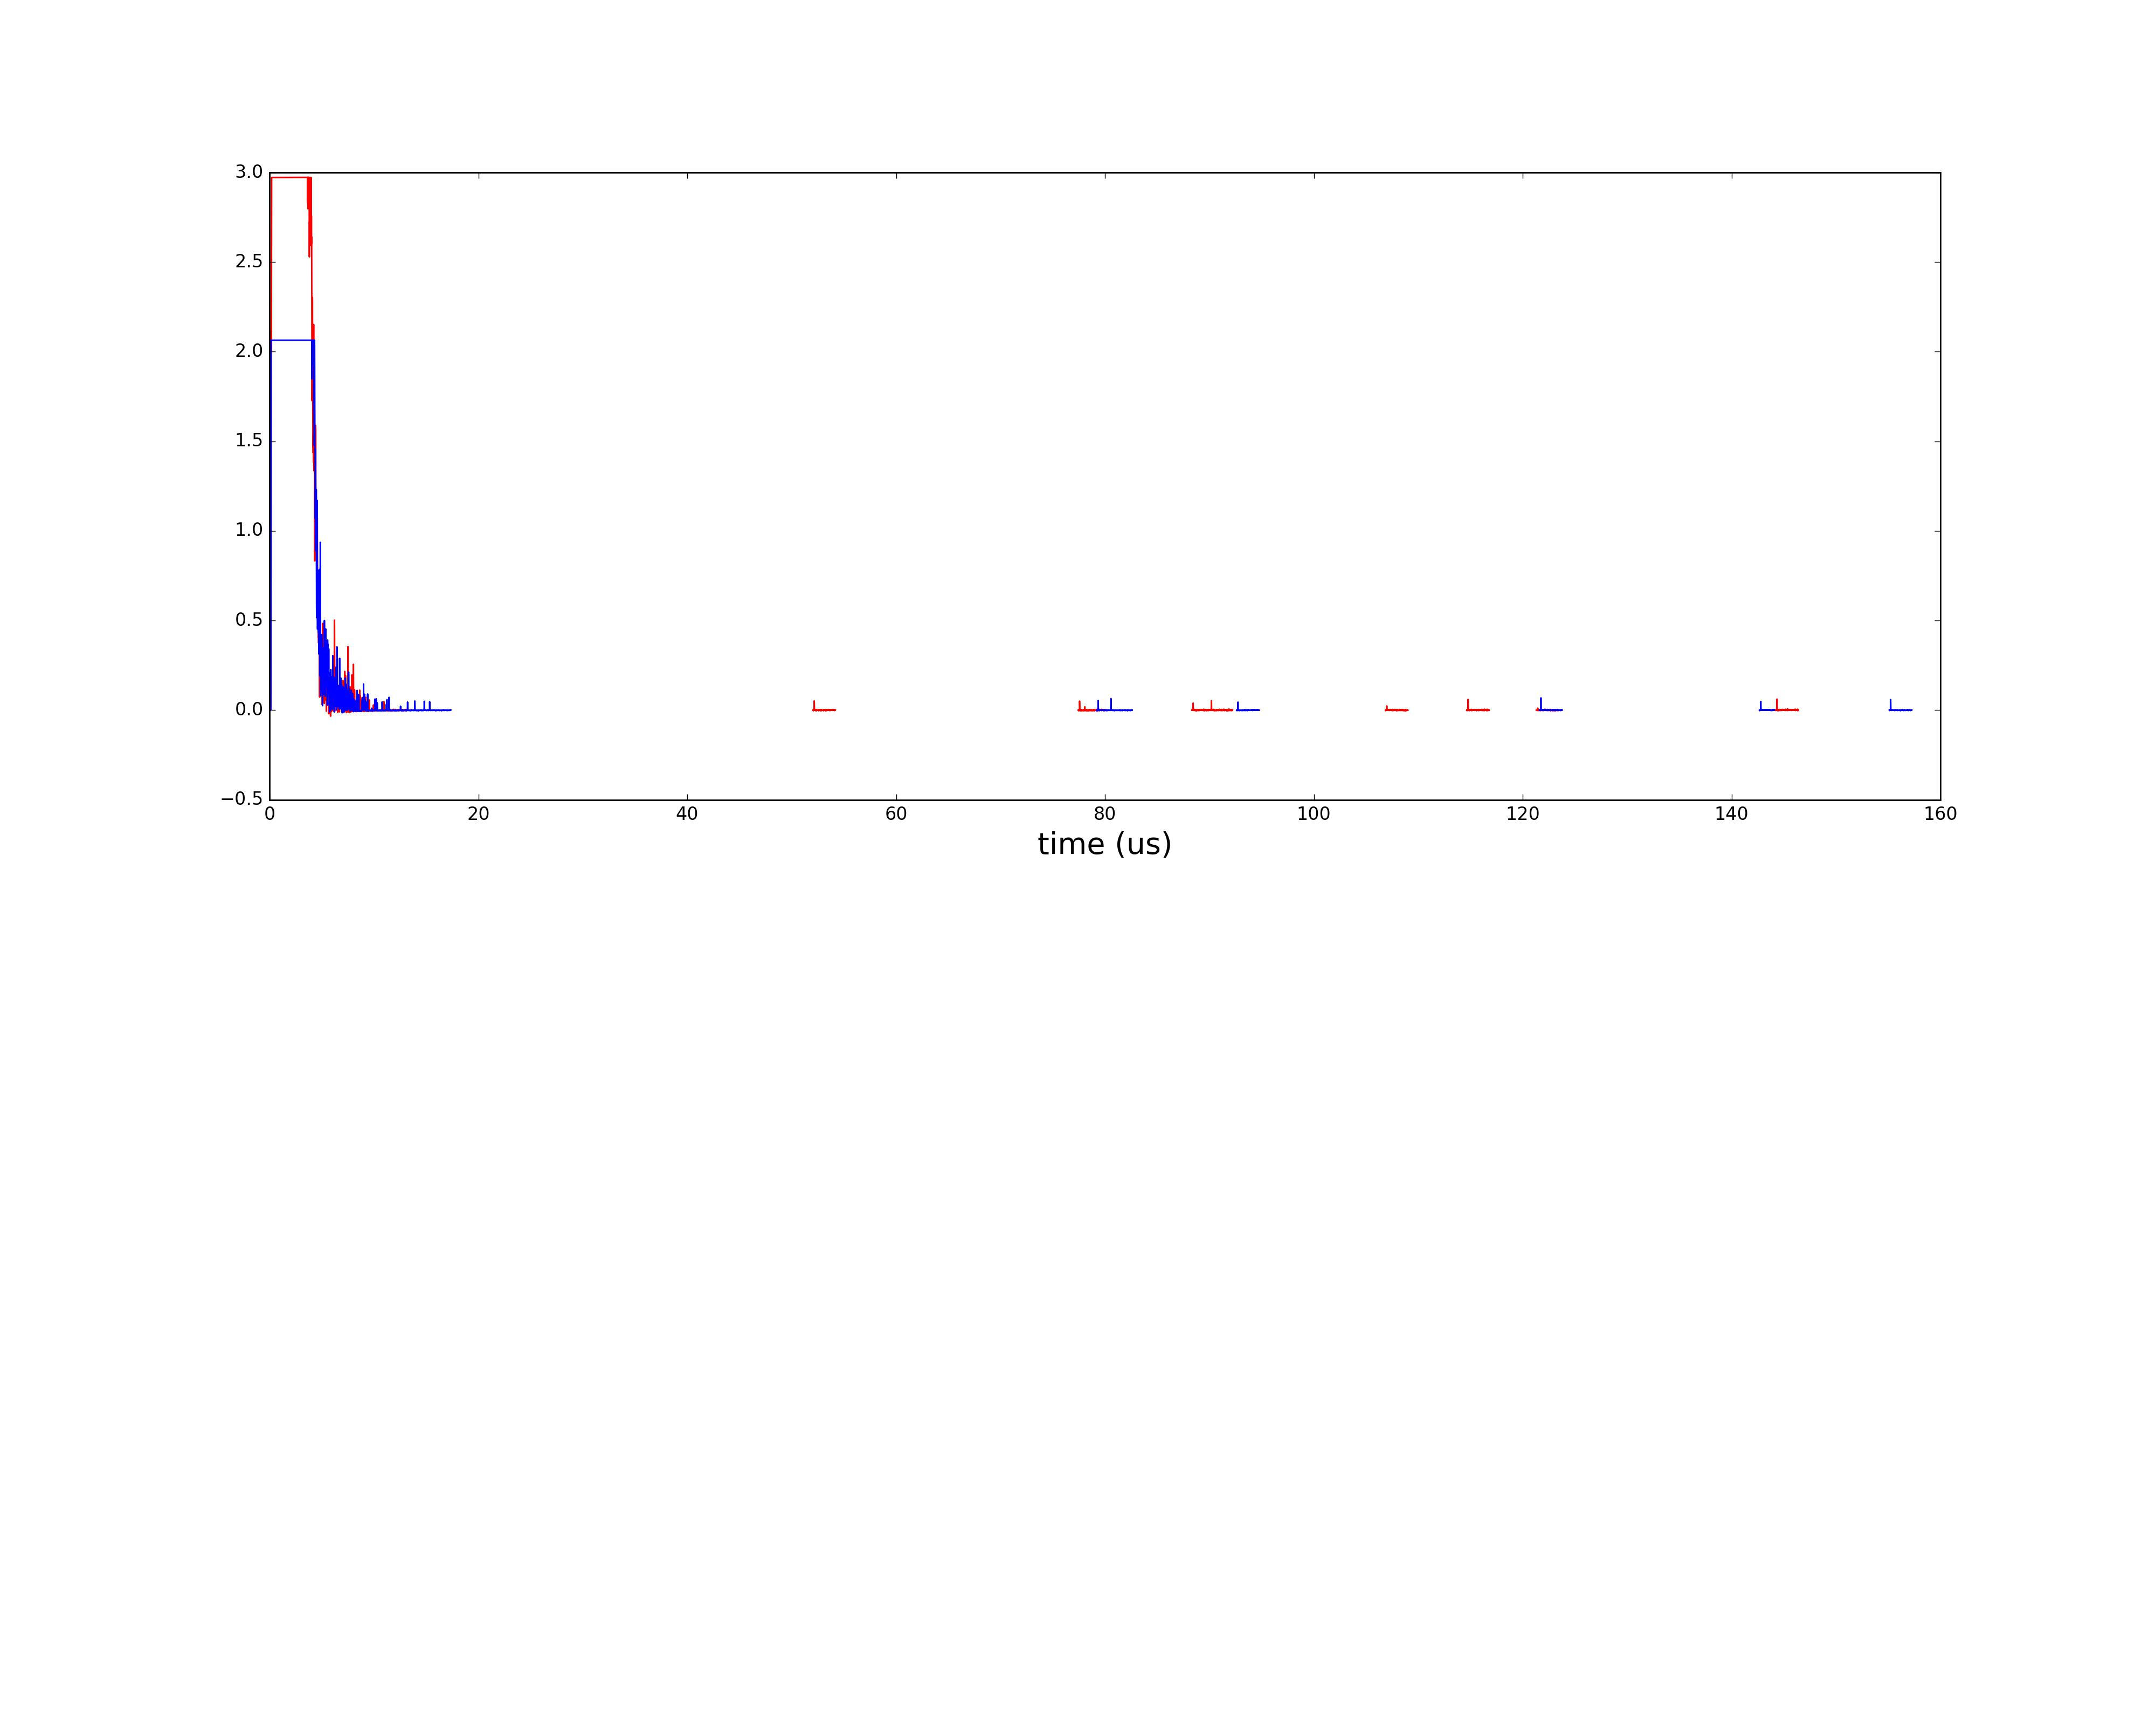
\includegraphics[width=0.8\textwidth,clip,trim={0 600 0 0}]
  {Figures/Ch10/SampleWaveforms/_64767_a_+6_0_g_-6_0_PlotCoinWaveforms_Plotid136198_.jpg}
  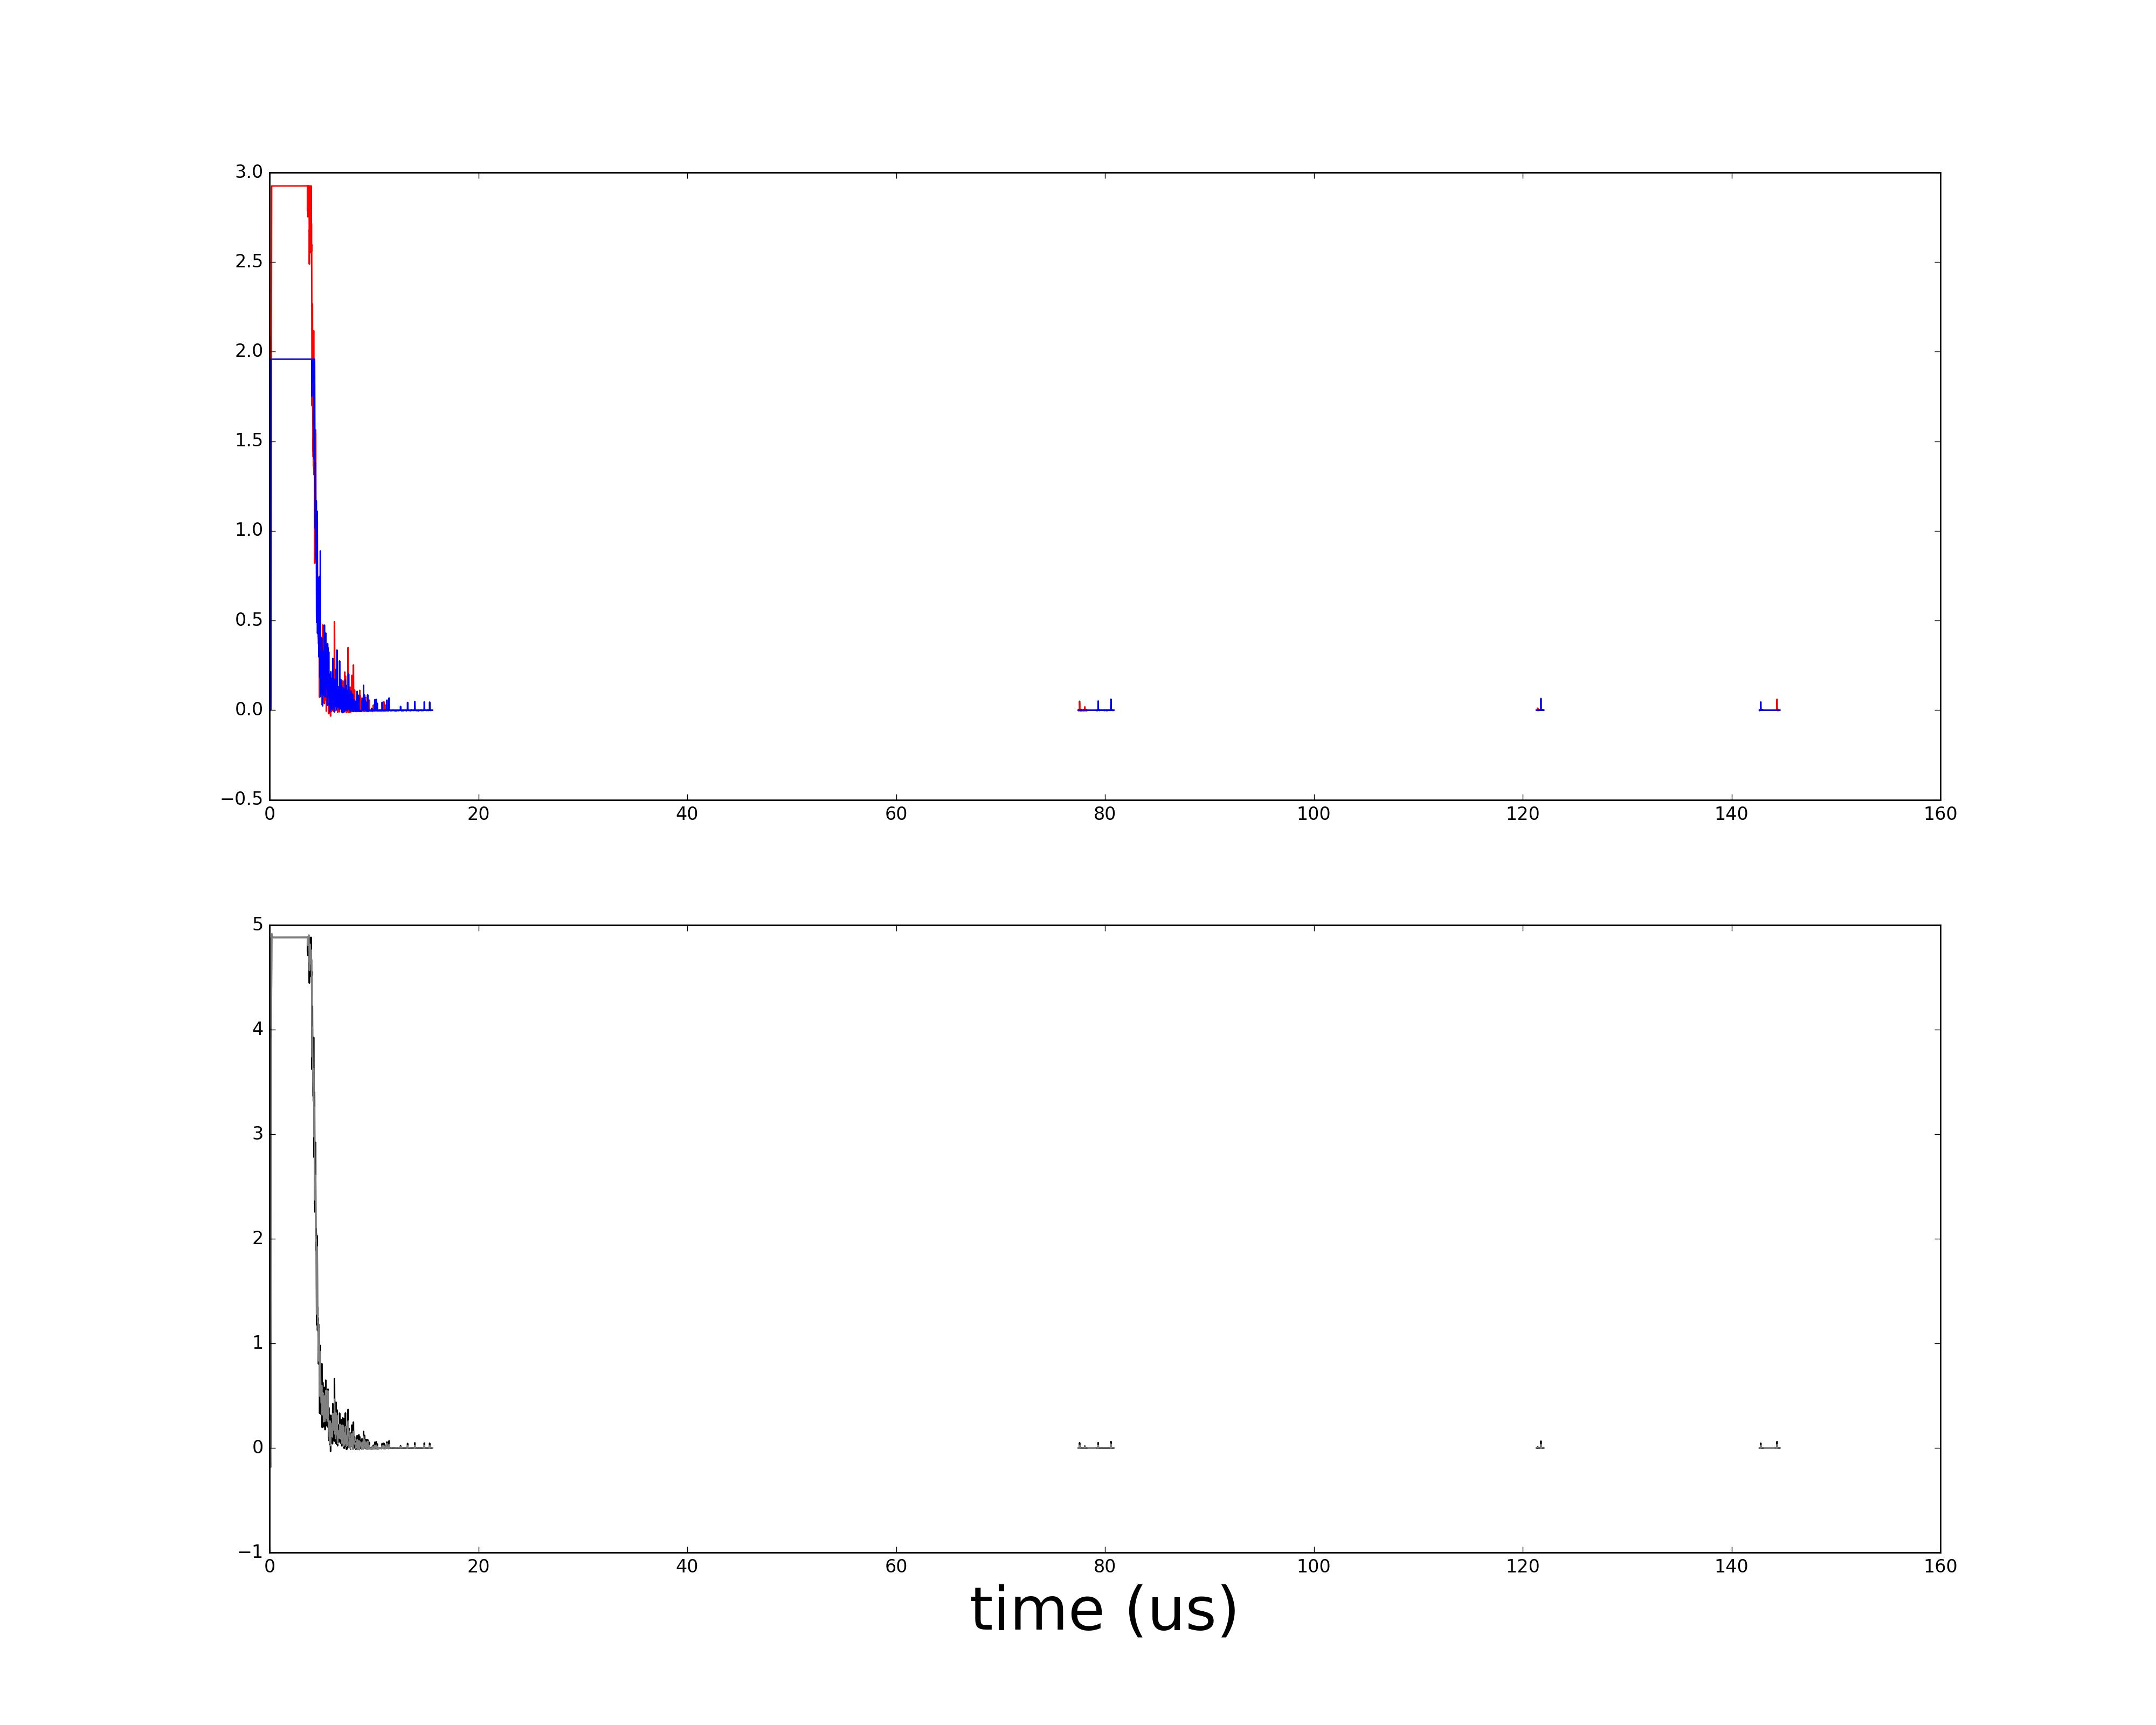
\includegraphics[width=0.8\textwidth,clip,trim={0 0 0 0}]
  {Figures/Ch10/SampleWaveforms/_64767_a_+6_0_g_-6_0_Cut33_big_pulse_PlotCoinWaveforms_104_.jpg}
  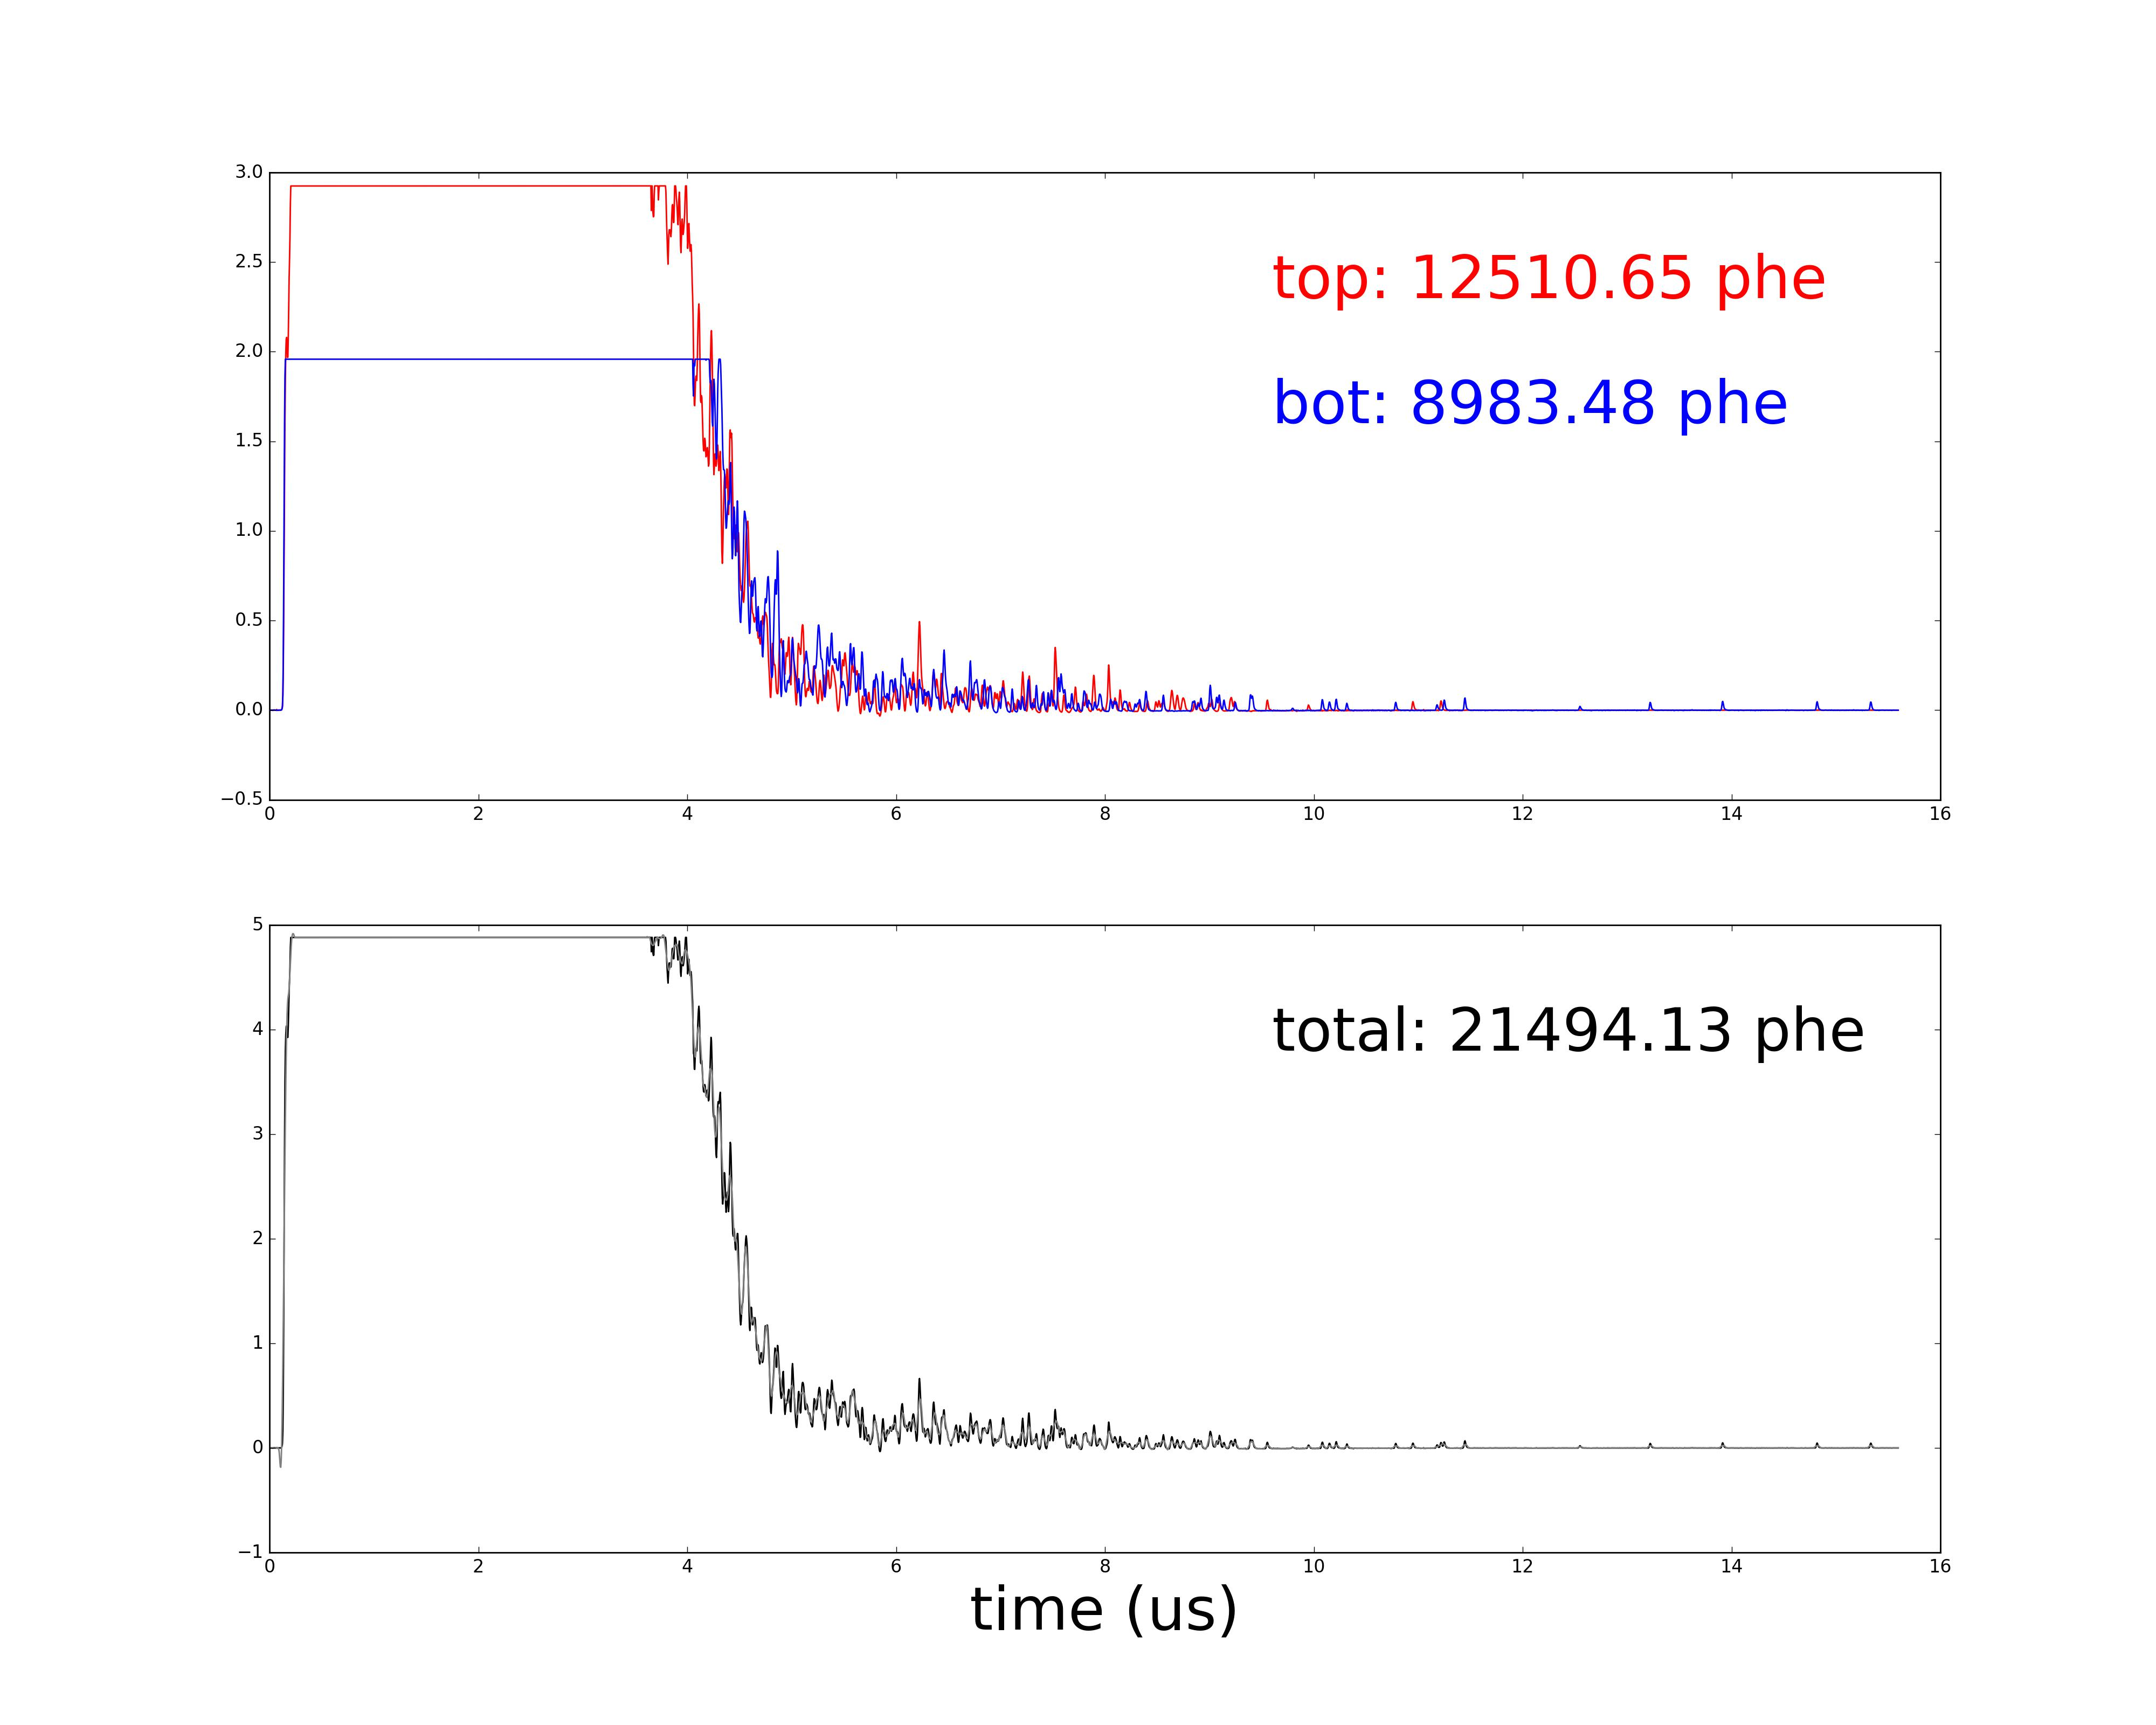
\includegraphics[width=0.35\textwidth,clip,trim={0 600 0 0}]
  {Figures/Ch10/SampleWaveforms/_64767_a_+6_0_g_-6_0_PlotCoinWaveforms_Plotid11162_.jpg}
  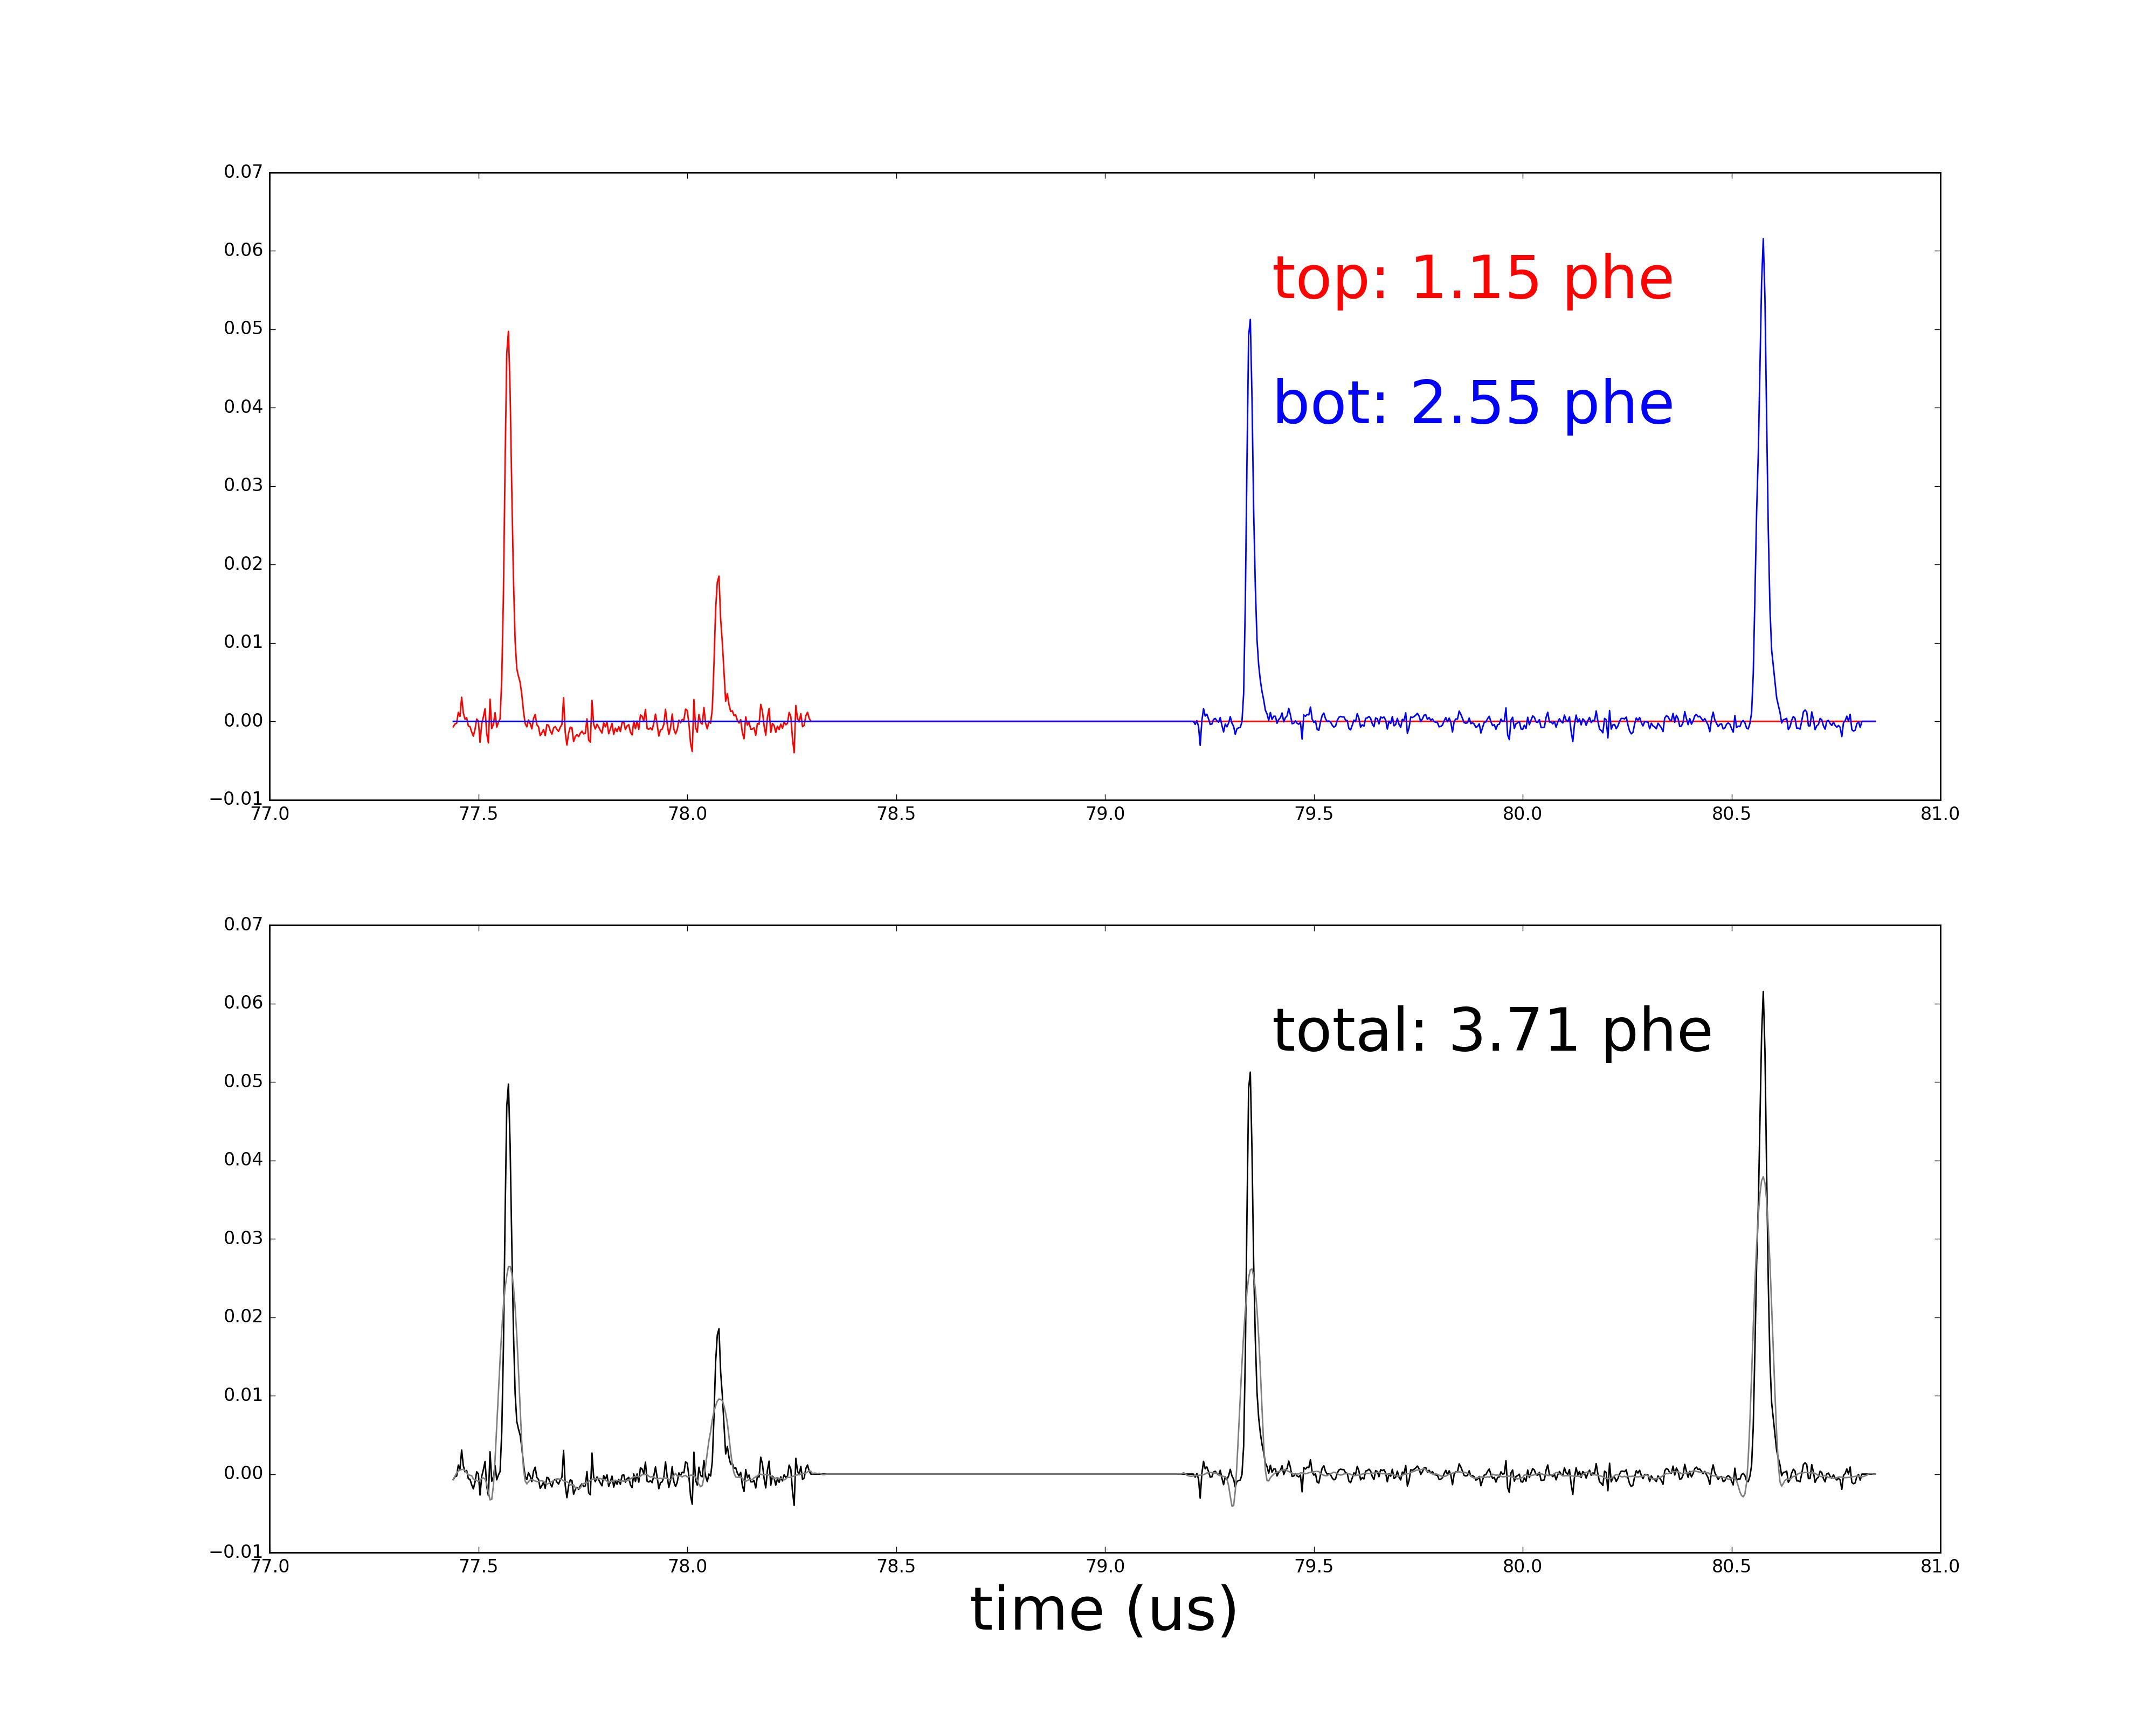
\includegraphics[width=0.35\textwidth,clip,trim={0 600 0 0}]
  {Figures/Ch10/SampleWaveforms/_64767_a_+6_0_g_-6_0_PlotCoinWaveforms_Plotid11163_.jpg}
  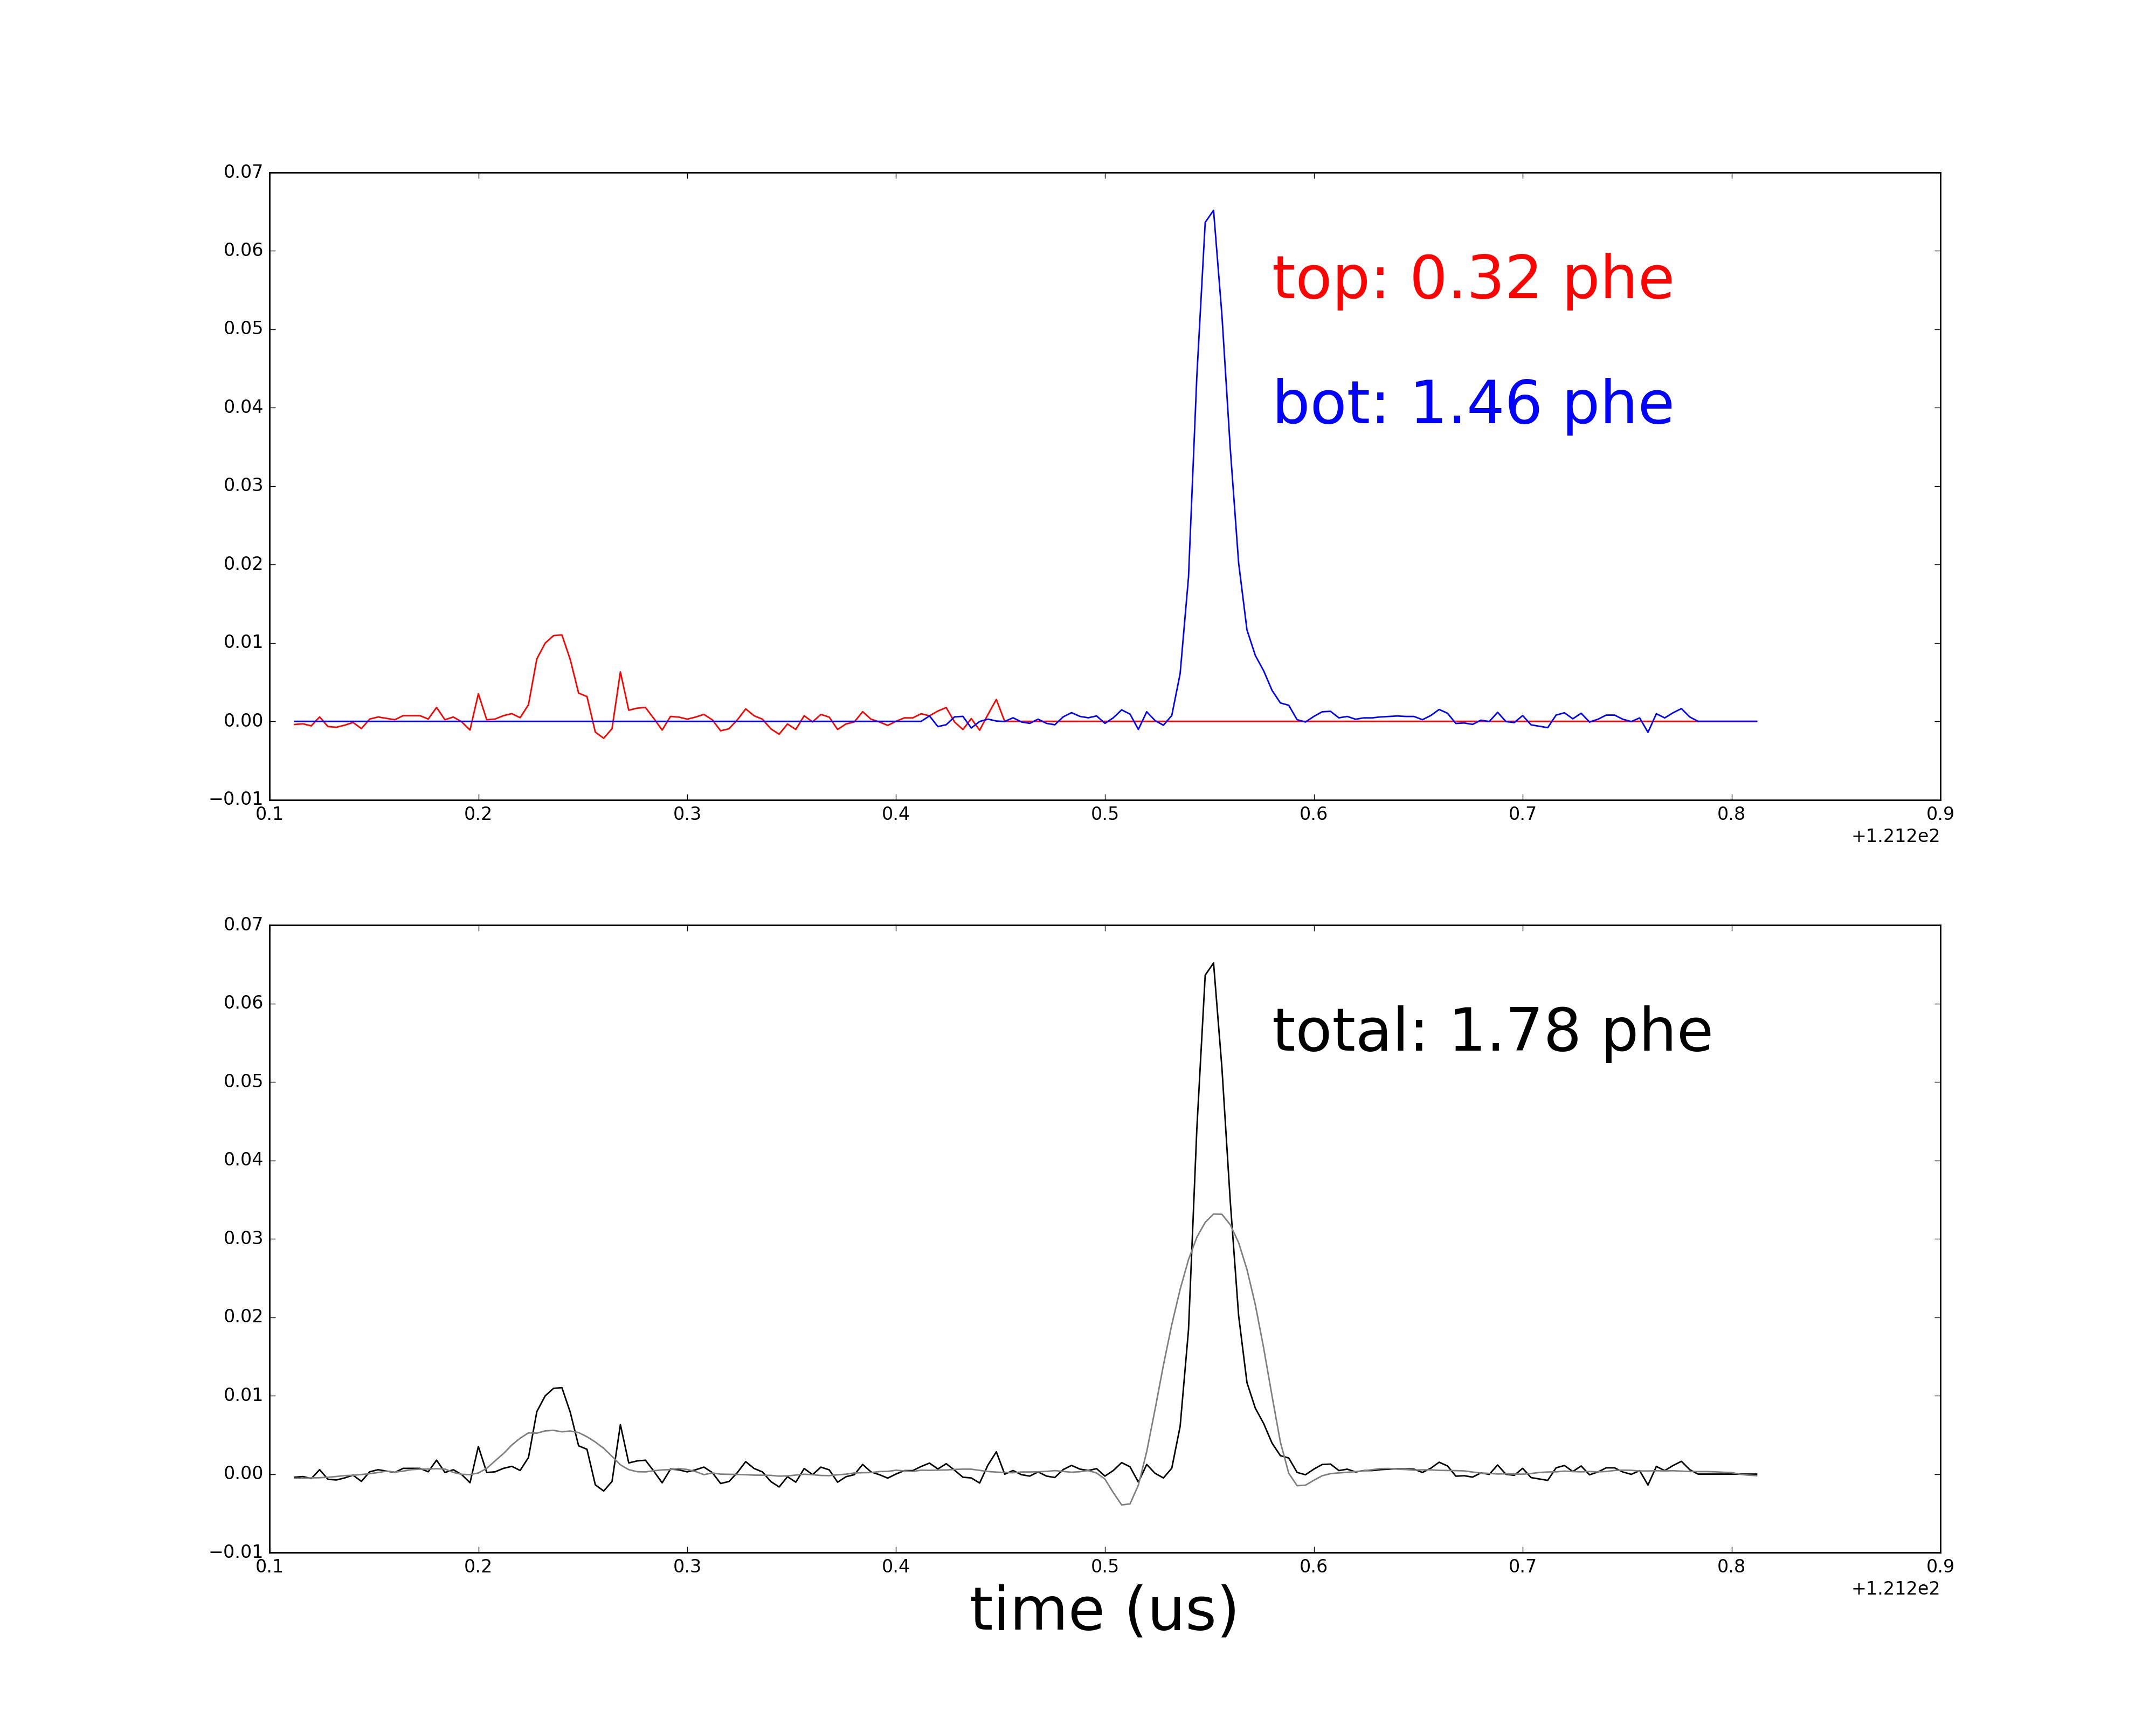
\includegraphics[width=0.35\textwidth,clip,trim={0 600 0 0}]
  {Figures/Ch10/SampleWaveforms/_64767_a_+6_0_g_-6_0_PlotCoinWaveforms_Plotid11164_.jpg}
  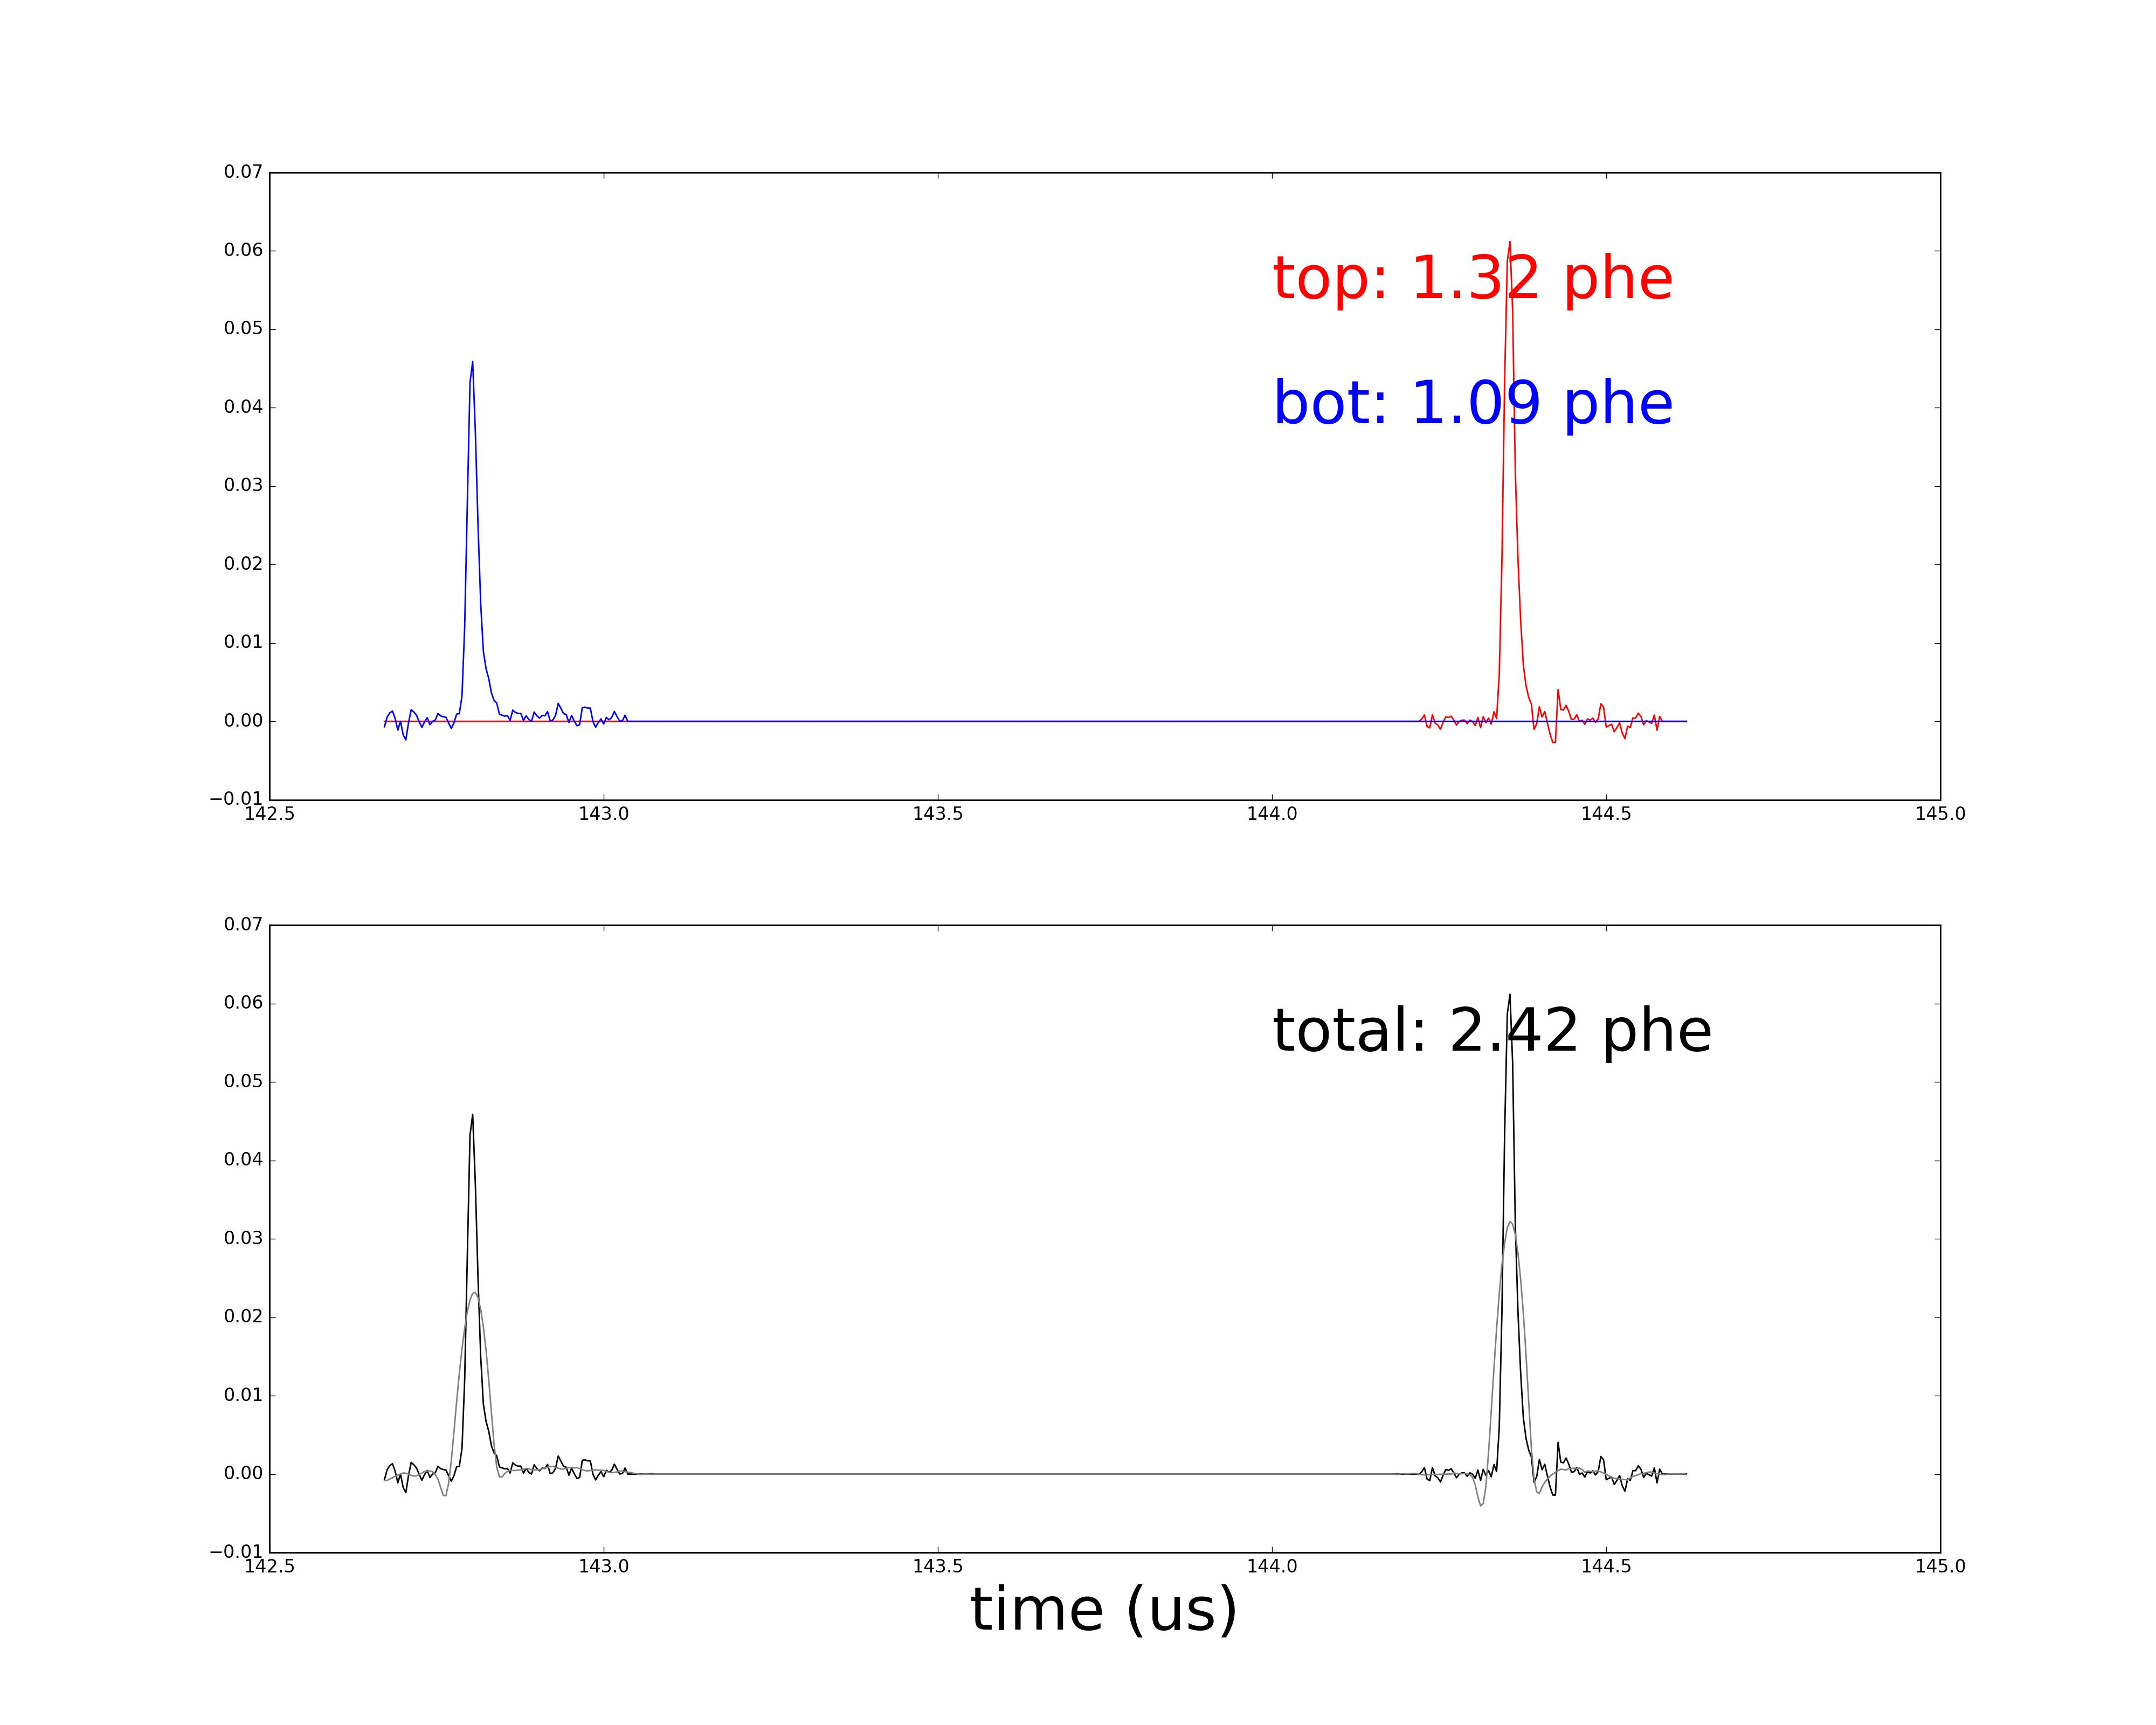
\includegraphics[width=0.35\textwidth,clip,trim={0 600 0 0}]
  {Figures/Ch10/SampleWaveforms/_64767_a_+6_0_g_-6_0_PlotCoinWaveforms_Plotid11165_.jpg}
  \caption{Photons after a big pulse. Top: all pulses recorded. Middle: coincidence pulses in top and bottom channels. Bottom: separate coincidence pulses. Red line is top PMT. Blue line is bottom PMT. Black line is the sum of top and bottom PMTs. }
  \label{fig: Photons after a big pulse}
\end{figure}
\end{center}

\section{Drift velocity calibration}

\begin{center}
\begin{figure}[!htbp]
\begin{tabular}{|l|*{1}{c|}}\hline

\makebox[0.45\textwidth]{$P = 0.5 bara, T = 290 K, n = 0.0208 mol/L$}&\makebox[0.45\textwidth]{$P = 1.0 bara, T = 290 K, n = 0.0417 mol/L$}\\\hline\hline        
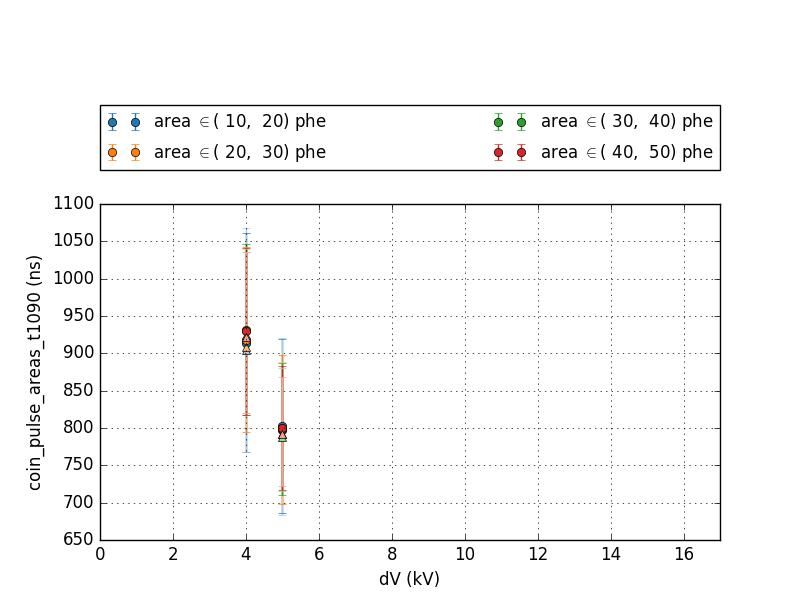
\includegraphics[width=0.45\textwidth,clip,trim={0 0 0 130}]{Figures/Ch10/cal_0500mbara_drift_time_cal.jpg} & 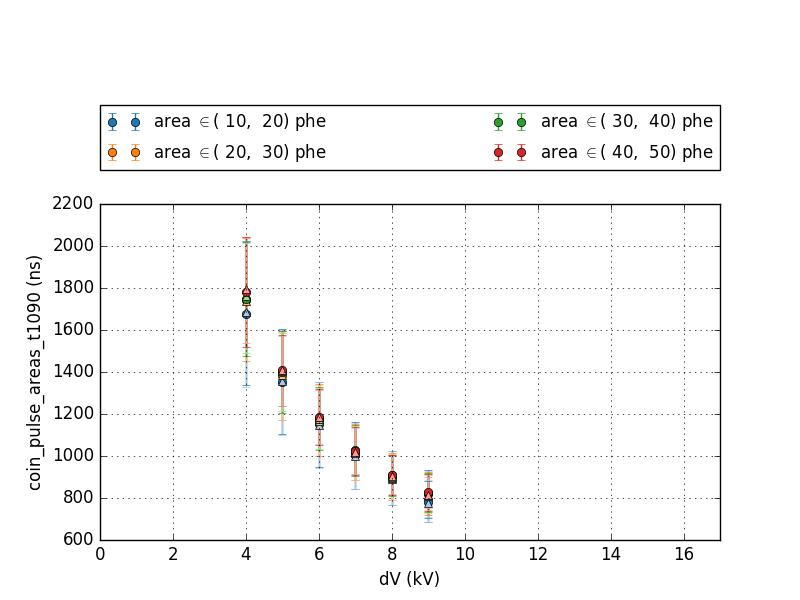
\includegraphics[width=0.45\textwidth ,clip,trim={0 0 0 130}]{Figures/Ch10/cal_1000mbara_drift_time_cal.jpg} \\ 
\multicolumn{1}{|m{0.45\textwidth}|}{}& \multicolumn{1}{m{0.45\textwidth}|}{}
\\\hline\hline

\makebox[0.45\textwidth]{$P = 1.5 bara, T = 290 K, n = 0.0627 mol/L$}&\makebox[0.45\textwidth]{$P = 2.0 bara, T = 290 K, n = 0.0839 mol/L$}\\\hline\hline        
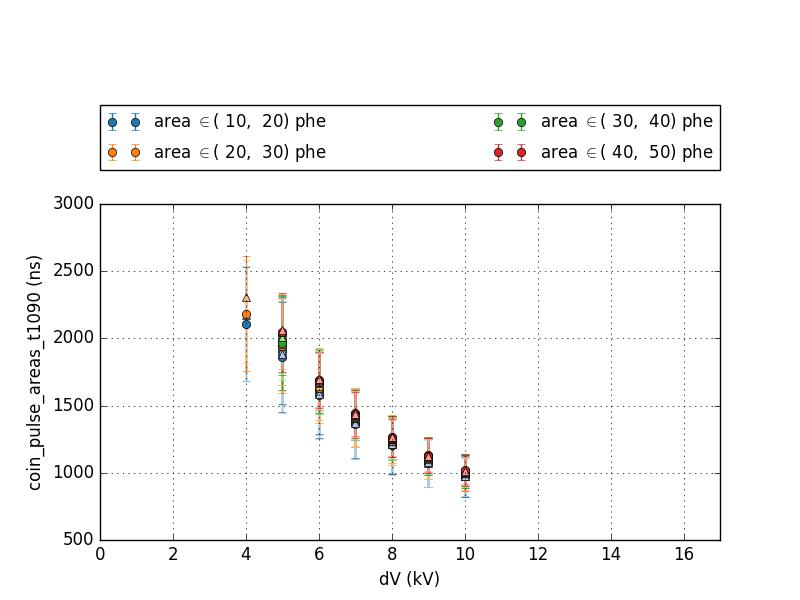
\includegraphics[width=0.45\textwidth,clip,trim={0 0 0 130}]{Figures/Ch10/cal_1500mbara_drift_time_cal.jpg} & 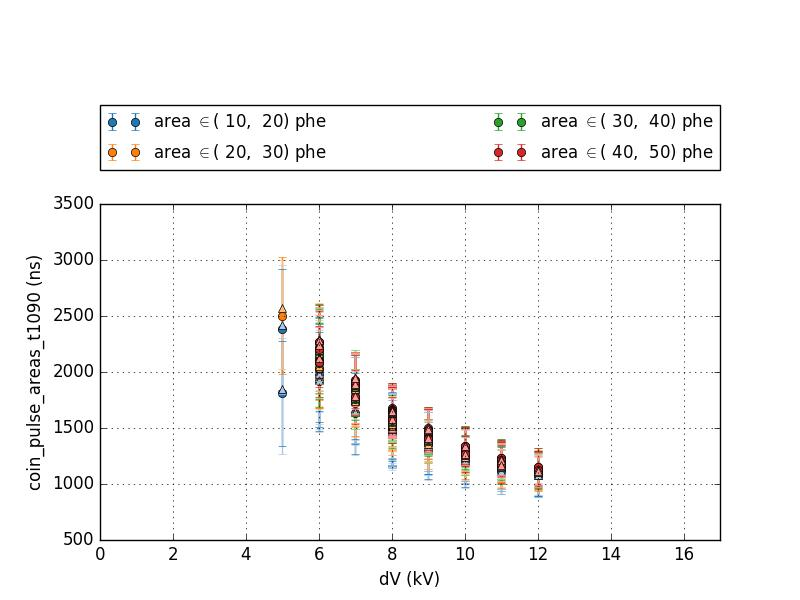
\includegraphics[width=0.45\textwidth ,clip,trim={0 0 0 130}]{Figures/Ch10/cal_2000mbara_drift_time_cal.jpg} \\ 
\multicolumn{1}{|m{0.45\textwidth}|}{}& \multicolumn{1}{m{0.45\textwidth}|}{}
\\\hline\hline

\makebox[0.45\textwidth]{$P = 2.5 bara, T = 290 K, n = 0.1052 mol/L$}&\makebox[0.45\textwidth]{$P = 3.0 bara, T = 290 K, n = 0.1266 mol/L$}\\\hline\hline        
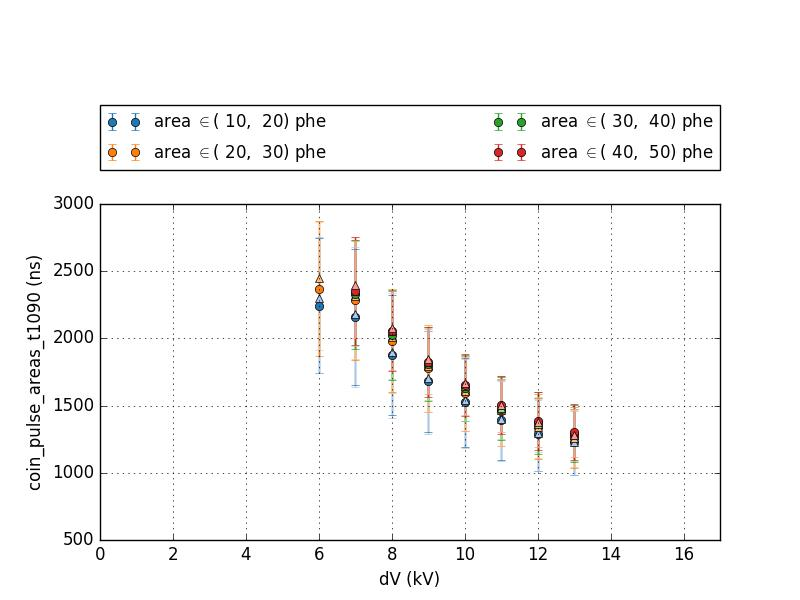
\includegraphics[width=0.45\textwidth,clip,trim={0 0 0 130}]{Figures/Ch10/cal_2500mbara_drift_time_cal.jpg} & 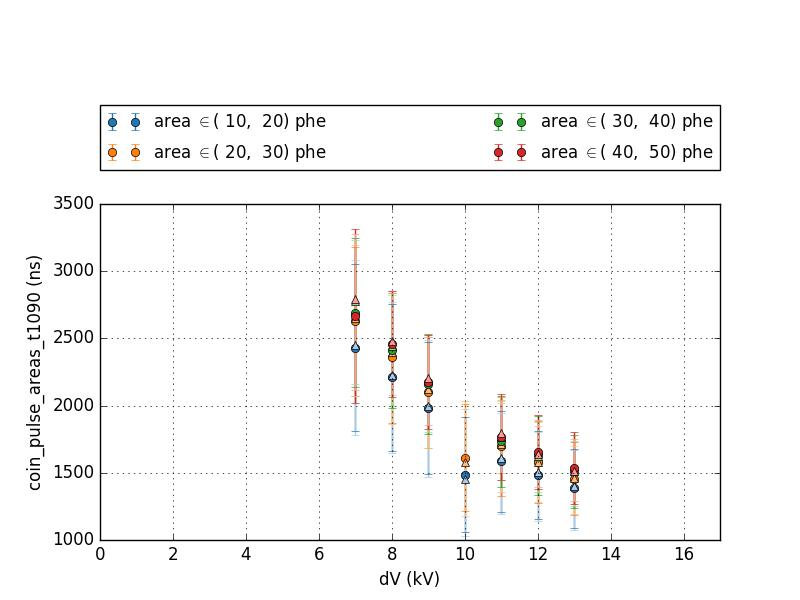
\includegraphics[width=0.45\textwidth ,clip,trim={0 0 0 130}]{Figures/Ch10/cal_3000mbara_drift_time_cal.jpg} \\ 
\multicolumn{1}{|m{0.45\textwidth}|}{}& \multicolumn{1}{m{0.45\textwidth}|}{}
\\\hline\hline

\makebox[0.45\textwidth]{$P = 3.5 bara, T = 290 K, n = 0.1481 mol/L$}&\makebox[0.45\textwidth]{$P = 3.4 bara, T = 290 K, n = 0.1438 mol/L$}\\\hline\hline        
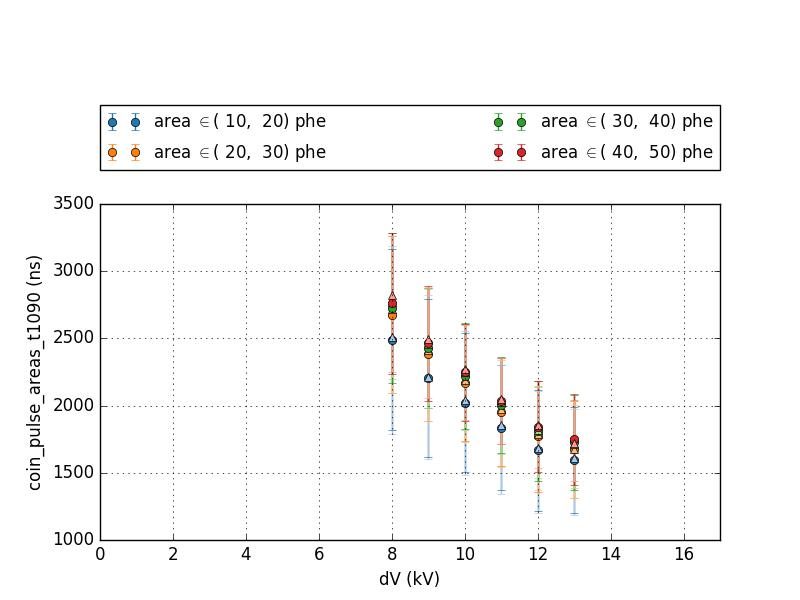
\includegraphics[width=0.45\textwidth,clip,trim={0 0 0 130}]{Figures/Ch10/cal_3500mbara_drift_time_cal.jpg} & 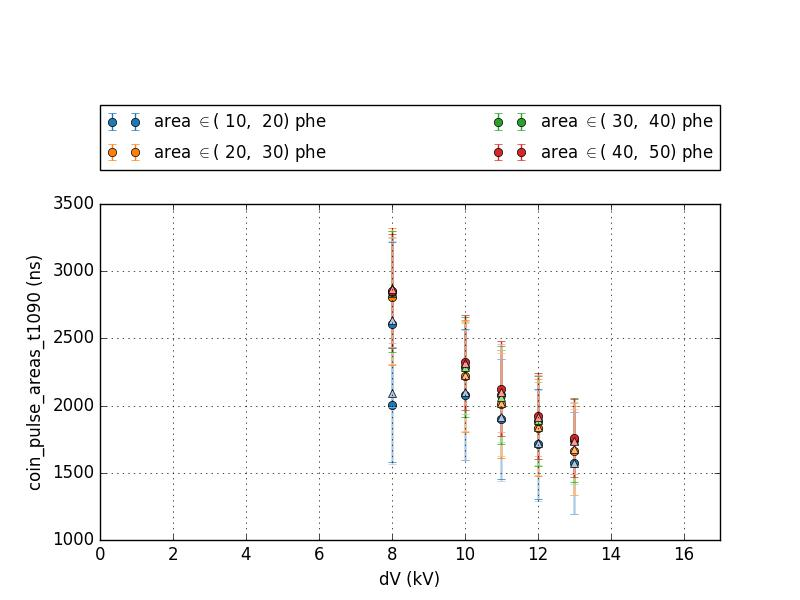
\includegraphics[width=0.45\textwidth ,clip,trim={0 0 0 130}]{Figures/Ch10/ShortTest_drift_time_cal.jpg} \\ 
\multicolumn{1}{|m{0.45\textwidth}|}{}& \multicolumn{1}{m{0.45\textwidth}|}{}
\\\hline
    \end{tabular}
    \label{drift t1090 calibration}
    \caption{Measured time difference between 10\% integrated area and 90\% integrated area ($t1090$). Solid circle: Mean and standard error. Triangle: Median and $14\%, 86\%$ percentile. Blue curve: 'coin\_pulse\_areas' $\in (10,20] phe$. Orange curve: 'coin\_pulse\_areas' $\in (20,30] phe$. Green curve: 'coin\_pulse\_areas' $\in (30,40] phe$. Red curve: 'coin\_pulse\_areas' $\in (40,50] phe$.}
\end{figure}

\begin{figure}[!htbp]
  \centering
  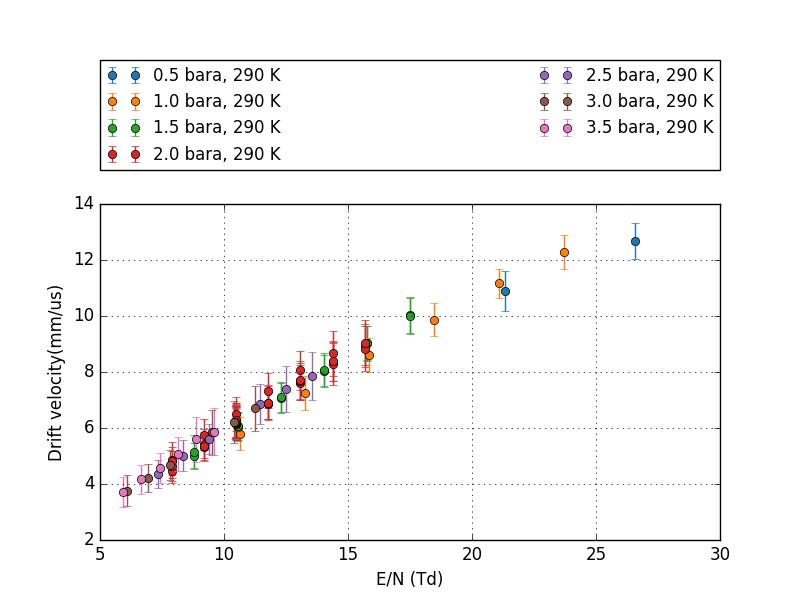
\includegraphics[width=0.9\textwidth,clip,trim={0 0 0 0}]
  {Figures/Ch10/drift_vel_cal_sum.jpg}
  \caption{Drift velocity}
  \label{fig: Drift velocity calibration}
\end{figure}
\end{center}


\section{Electron emission changing over time}
During the experiment, an increasing of electron emission over time was observed. And the reason of this phenomenon is possibly the rearranging of the electric field in the detector around the grid wires. Because of the difference between the drift velocity of the electrons and the ions. Electrons moves faster thus vanish earlier comparing to ions. This results in a positive charge environment in the detector especially around the grid wires that is being studied. The increasing of the density of ions would enhance the electric field around the grid wires, thus increase the electron emission from them.
For clearly studying this problem, a series of dataset were taken every $10$ minutes with operating the anode and the gate grid steadily at $+4,-4kV$. Fig: \ref{fig: Emission changing during the experiment} shows the rate changing over time during the experiment. Studies shows that the emission enhancement was stronger at coincidence pulse area smaller than $30$ phe and was very weak at larger coincidence pulse area. This indicates that the excess events seen may come from the enhancement of single electron emission and the light accompany with it.  
\begin{figure}[!htbp]
  \centering
  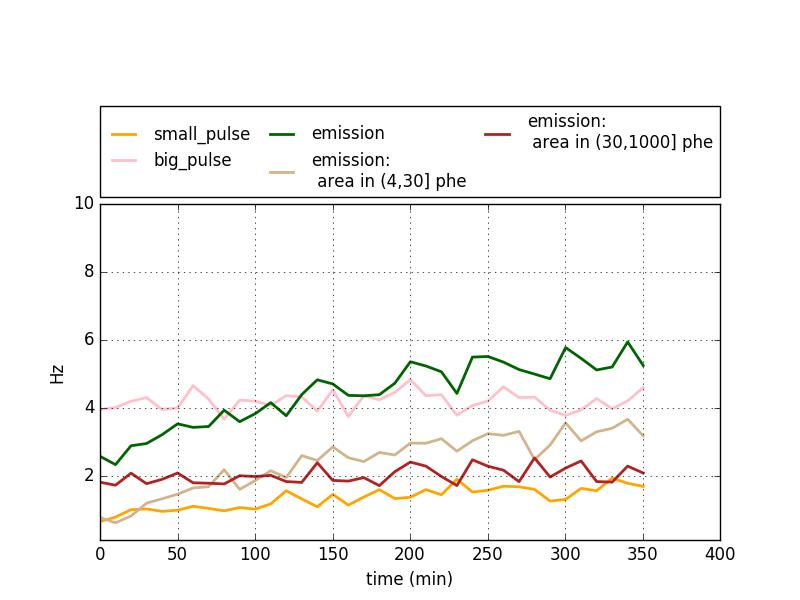
\includegraphics[width=0.9\textwidth,clip,trim={0 0 0 170}]
  {Figures/Ch10/a4gn4_coin_pop_plot_important.jpg}
  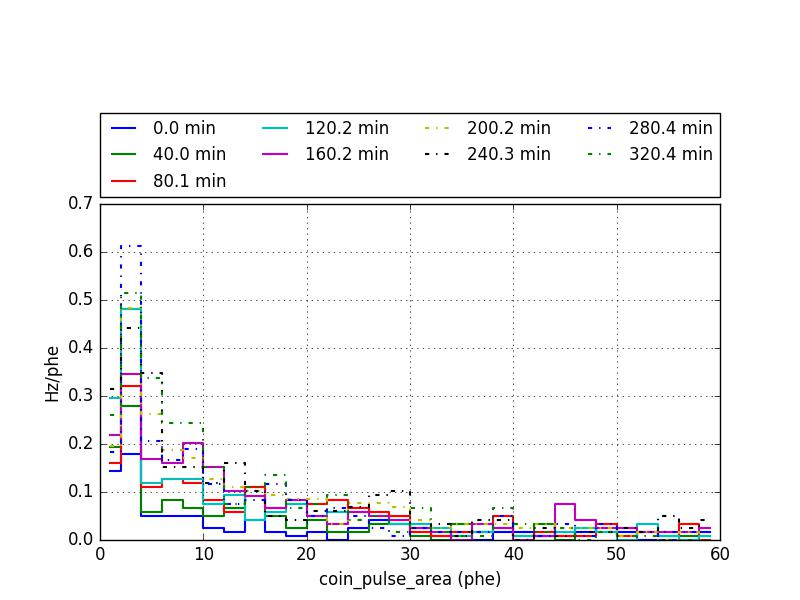
\includegraphics[width=0.9\textwidth]
  {Figures/Ch10/a4gn4_hist_others_evolve_wavearea.jpg}
  \caption{Top: emission rate changing over time during the experiment with $v_a=+4kV, \quad v_g=-4 kV$. orange: area $\in$ (0,4] phe, tan: area $\in$ (4,30] phe, red: area $\in$ (30,1000] phe, pink: area $\in$ (1000, $\infty$) phe, green: sum of tan and red curve. Bottom: emission rate at different area changing over time.}
  \label{fig: Emission changing during the experiment}
\end{figure}





\section{The influence of impurity in xenon}

\section{The influence of long operation duration}

\section{The influence of grid passivations}
















































\section{Discussion about LZ grids}


\begin{center} 
  \begin{tabular}{ | l | c  c  c c c  r |}
    \hline 
    Grid Name & Top PMT & Anode & Gate & Cath & Bottom & Bot PMT\\ 
	Location from liquid surface (mm) & 78 & 8 & -5 & -1461 & -1598.5 & -1608.5\\
    Operation Voltage(kV) & -1.5 & 5.75 & -5.75 & -50 & -1.5 & -1.5 \\
	Wire Pitch (mm)& NA & 2.5 & 5 & 5 & 5 & NA\\ 
	Wire Diameter (um) & NA & 100 & 75 & 100 & 75 & NA\\
    Tension (N) & NA & 2.5 & 2.5 & 2.5 & 2.5 & NA \\
    Deflection (mm) & NA & 0.59 & 0.61 & 0.19 & 0.19 & NA \\
    Wire Surface ($m^2$) & 1.665 & 0.423 & 0.159 & 0.212  & 0.158 & 1.665 \\
    Average Surface Field (kV/cm) & 1.0 & 43.7 & -51.0 & -30.1 & 33.1 & 0.4 \\
    Wire Top max Surface Field (kV/cm) & NA & 39.2 & -53.7 & -28.5 & 35 & 0.3 \\ 
	Wire Bot max Surface Field (kV/cm) & 1.0 & -48.2 & 48.3 & 31.6 & -31.2 & NA \\
 \\ 
  \end{tabular}
 LZ grids parameters
\end{center}





